\chapter{C05, 7. évfolyam}
\section{Kombinatorika}

\subsection*{2005.09.13.}
\begin{enumerate}
\item Állíts össze 15 dominóból egy $5\times 6$-os
téglalapot úgy, hogy a téglalap bármelyik oldalával
párhuzamos egyenes minden esetben legalább egy dominót kettévágjon!
\item Az előző feladat eredménye alapján 20 dominóból állíts össze $5\times 8$-as téglalapot ugyanilyen módon!
\item 24 dominóból állíts össze $6\times 8$-as téglalapot az előző két feladatban megismert tulajdonsággal!
\item Összeállítható-e téglalap az ötféle \textit{tetraminóból} (mindegyikből csak egy példányunk van)?
\item Állíts össze egy $6\times 10$-es téglalapot
a 12 \textit{pentaminóból} (mindegyikből csak egy példányunk van)?
\item A $8\times 8$-as sakktábla egyik sarokmezőjét kihagyjuk. Lefedhető-e a megmaradt rész 21 darab ilyen \textit{tri\-minóval}: 
\tikz[x=0.2cm,y=0.2cm]{
\draw (0.,4.)-- (3.,4.);
\draw (3.,4.)-- (3.,3.);
\draw (3.,3.)-- (0.,3.);
\draw (0.,3.)-- (0.,4.);
\draw (1.,4.)-- (1.,3.);
\draw (2.,4.)-- (2.,3.);
}
?
\end{enumerate}

\subsection*{2005.09.15.}
\begin{enumerate}
\item Lefedhető-e a szokásos $8\times 8$-as sakktábla 15 T alakú és egy
\tikz[x=0.2cm,y=0.2cm]{
\draw (0.,0.)-- (2.,0.);
\draw (2.,0.)-- (2.,2.);
\draw (2.,2.)-- (0.,2.);
\draw (0.,2.)-- (0.,0.);
\draw (1.,0.)-- (1.,2.);
\draw (0.,1.)-- (2.,1.);
}
alakú tetraminóval?
\item Állíts össze a 12 pentaminóból $5\times 12$-es
téglalapot!
\item A sakktábla 4 sarokmezőjét kivágtuk.
A megmaradt részt fedjétek le a 12 pentaminóval!
\item A 12 pentaminóból állíts össze 3 darab $7\times 3$-as téglalapot úgy, hogy mindegyik téglalapból 1 mező üresen marad! 
\item A $8\times 8$-as sakktáblán jelölj ki 16 mezőt úgy, hogy a kimaradt részre ne lehessen letenni a következő pentaminókat: U, Y, I, L.
\end{enumerate}


\subsection*{2005.09.20.}
\begin{enumerate}
\item  Legfeljebb hány bástya helyezhető el a sakktáblán úgy, hogy egyik se üsse a másikat?
\item Legfeljebb hány futó helyezhető el a sakktáblán úgy, hogy egyik se üsse a másikat?
\item Legfeljebb hány király helyezhető el a sakktáblán úgy, hogy egyik se üsse a másikat?
\item Legfeljebb hány ló helyezhető el a sakktáblán úgy, hogy egyik se üsse a másikat?
\item Legfeljebb hány királynő helyezhető el a sakktáblán úgy, hogy egyik se üsse a másikat?
\item Legfeljebb hány
\begin{abcn}{5}
\item királyt;
\item bástyát;
\item futót;
\item lovat;
\item királynőt
\end{abcn}
kell elhelyezni a sakktáblán úgy, hogy minden
szabad mezőt ütés alatt tartsanak?
\end{enumerate}


\subsection*{2005.09.21.}
\begin{enumerate}
\item Egy kocka lapjait pirosra és kékre festjük. Hányféleképpen lehetséges ez, ha az elmozgatással egymásba vihető színezéseket nem tekintjük különbözőeknek?

\item Legfeljebb hány részre osztja a síkot 3 egyenes, 4 egyenes, 5 egyenes?

\item Egy négyzetet fel lehet-e darabolni 4, 6, 7, 8 négyzetre?

\item Egy $8 \times 8$-as sakktábla bal alsó sarkából el lehet-e jutni a jobb felső sarokba úgy, hogy közben minden sorba pontosan egyszer lépünk?

\item Egy $8 \times 8$-as sakktábla egyik mezőjét letakarjuk. Mutassuk meg, hogy a maradék rész lefedhető 21 darab
\tikz[x=0.2cm,y=0.2cm]{
\draw (-3.,5.)-- (-3.,3.);
\draw (-3.,3.)-- (-1.,3.);
\draw (-1.,3.)-- (-1.,4.);
\draw (-1.,4.)-- (-3.,4.);
\draw (-2.,5.)-- (-2.,3.);
\draw (-3.,5.)-- (-2.,5.);}
alakzattal.

\item Egy kockát fel lehet-e darabolni 27, 34, 90 kisebb kockára?

\item Adott a síkon 8 egyenes. Legfeljebb hány metszéspontjuk lehet?

\end{enumerate}


\subsection*{2005.09.27.}
\begin{enumerate}
\item Hány olyan háromjegyű szám van, amelynek jegyei között csak az 1, 2, 3 szerepel?

\item Hány olyan háromjegyű szám van, amelynek jegyei között csak a 0, 1, 2, 3, szerepel?

\item Hány olyan ötjegyű páros szám van, amelynek jegyei között nincs 5-nél nagyobb számjegy?

\item Hányféleképpen választhatunk ki az 1 és 10 közti egész számokból három számot?

\item Hány olyan téglatest van, amelynek élei egész hosszúságúak és legfeljebb 10 egység a hosszuk?

\item Egy piros és egy zöld kockával dobunk, leírjuk egymás mellé a kapott eredményt. Hányféle kétjegyű számot kaphatunk?

\item Hányféleképpen választhatunk ki az első 30 pozitív egész számból hármat úgy, hogy az összegük osztható legyen 3-mal?
\end{enumerate}


\subsection*{2005.09.28.}
\begin{enumerate}
\item Hány olyan 0001 és 9999 közötti egész szám van, amelyben két jegy összege megegyezik a harmadik és a negyedik jegy összegével?

\item Mennyi az 1, 2, 3, 4, 5, 6 számjegyekkel felírható hatjegyű számok összege?

\item Legfeljebb hány metszéspontot határoznak meg a konvex 7-szög, konvex 8-szög átlói?

\item Hány átlója van egy konvex 7, 8, 9-szögnek, 
$n$-szögnek?

\item Hány olyan téglatest van, amelynek az élei egész hosszúságúak és 1 és 20 közé esnek?

\item Hány olyan 4 jegyű szám van, amelynek a számjegyei 1,2,3 közül kerülnek ki, és osztható 
3-mal?
\end{enumerate}


\subsection*{2005.09.29.}
\begin{enumerate}
\item Mennyi az 1, 2, 3, 4 számjegyekkel felírható négyjegyű számok összege?

\item Hány 4-gyel osztható, 4-jegyű szám készíthető az 1, 2, 3, 4, 5 számjegyekből, ha ezek mindegyike többször is felhasználható?

\item Hány különböző forgalmi rendszám készíthető, ha egy rendszám 3 betűből és 3 számjegyből áll, és 26 betűből lehet választani, más megkötés nincs.

\item Hányféleképpen lehet a 10-et pozitív egész számok összegére bontani, ha a sorrendben különböző felbontásokat különbözőnek tekintjük? És a 20-at?

\item Hányféleképpen lehet a 10-et nemnegatív egész számok összegére bontani, ha a sorrendben különböző felbontásokat is különbözőnek tekintjük? És a 20-at?
\end{enumerate}


\subsection*{2005.10.05.}
\begin{enumerate}
\item Az 5-nél nem nagyobb számjegyekkel elkészítjük az összes 4 jegyű számot, amelyekben nincs ismétlődő számjegy. Mennyi ezek összege?

\item Egy konvex tízszög átlói legfeljebb hány metszéspontot határoznak meg a sokszög belsejében?

\item Egy piros és egy zöld dobókockával dobunk, a dobott számokat összeadjuk. Milyen számokat kaphatunk és melyiket hányféleképpen?

\item Egy 10 lépcsőfokból álló lépcsőn úgy mehetünk fel, hogy egyszerre 1 vagy 2 lépcsőfokot lépük. Hányféleképpen mehetünk fel?

\item Hány részre osztják a teret a kocka lapsíkjai?

\item Hány olyan ötjegyű szám van, amelyekben az 5-nél nem nagyobb számjegyek szerepelnek és osztható 4-gyel?
\end{enumerate}


\subsection*{2005.10.06. -- Kombinatorika dolgozat}
\begin{enumerate}
\item Mennyi az 1, 2, 3, 4 számjegyekből készíthető
négyjegyű számok összege? Minden számjegy csak egyszer szerepelhet a számban.
\item Hány olyan 4-jegyű szám van, amelyben a számjegyek összege páros?
\item Legfeljebb hány részre osztja a síkot 6 egyenes?
\item Hányféleképpen lehet a 12-t három pozitív egész szám összegére bontani, ha a csak sorrendben különböző felbontásokat is különbözőnek tekintjük?
\item Egy kocka lapjait három színnel, pirossal, kékkel és zölddel színezzük. A színezéshez mind a három színt felhasználjuk.
Hányféle kockát kaphatunk, ha az elforgatással egymásba vihetőket nem tekintjük különbözőnek?
\end{enumerate}


\section{Számelmélet}

\subsection*{2005.10.11.}
\begin{enumerate}
\item Adjunk meg 9 egymást követő összetett számot!

\item Meg lehet-e adni 20 egymást követő összetett számot?

\item Meg lehet-e adni 100 egymást követő összetett számot?

\item Bizonyítsuk be a 9-cel való oszthatóság szabályát!

\item Bizonyítsuk be a 3-mal való oszthatóság szabályát!

\item Igazoljuk, hogy bármely pozitív egész $n$ számra igaz, hogy $n^3-n$ osztható 6-tal!

\item Bizonyítsuk be, hogy ha egy $p$ törzsszám nagyobb mint 3, akkor 6-tal osztva 5 vagy 1 maradékot ad!

\item Mi a 11-gyel való oszthatósági szabály?

\end{enumerate}

\subsection*{2005.10.13.}
\begin{enumerate}
\item Lehet-e egy tízes számrendszerben felírt pozitív egész szám számjegyeinek szorzata 111?

\item Melyik az a legnagyobb természetes szám, amelynek számjegyei 7-nél kisebb és 0-nál nagyobb számjegyek, minden számjegy csak egyszer szerepel benne és osztható 12-vel?

\item AZ 1, 2, 3, 4, 5, 6 számjegyekkel felírt hatjegyű számok között lehet-e négyzetszám? (Minden számjegy csak egyszer szerepelhet!)

\item Öt egymást követő pozitív egész szám szorzata milyen számjegyre végződik?

\item Öt egymást követő pozitív \underline {páratlan} szám szorzata milyen számjegyre végződik?

\item Négy egymást követő egész szám szorzata 3024. Mik ezek a számok?

\item Lehet-e 10 egymást követő pozitív egész szám összege osztható 10-zel?

\item Adjuk meg a 45-nek egy olyan többszörösét, amiben csak a 0 és a 8 számjegy szerepel!
\end{enumerate}

\subsection*{2005.10.18.}
\begin{enumerate}
\item Íjuk át a következő, tízes számrendszerben megadott számokat 7 alapú és 9 alapú számrendszerbe: $$14,\qquad 27,\qquad 135,\qquad 2005.$$

\item Írjuk át a következő 7 alapú számrendszerben megadott számot 9 alapú számrendszerbe: $30514_7$.

\item Milyen alapú számrendszerben igaz a következő egyenlőség: 

\begin{abc2}

	\item $190_{10}=231_{x}$;
	\item $884_{10}=1182_x$?
 
\end{abc2}

\item A tízes számrendszerben $2\cdot 9=18$ és $9^2=81$, ugyanazokból a számjegyekből áll, csak fordított sorrendben. Igazoljuk, hogy bármely $n$ alapú számrendszerben az $n-1$ kétszerese és négyzete is ugyan azokból a számjegyekből áll, csak fordított sorrendben!

\item Milyen alapú számrendszerben érvényes a következő szorzás?

\begin{tabular}{ccccccc}
  &1&2&1&$\cdot$&2&2\\
  \cline{1-4}
  & 2 & 4 & 2 & & & \\
2 & 4 & 2 &   & & & \\
  \cline{1-4}
3 & 2 & 1 & 2 & & & 
\end{tabular}

\end{enumerate}

\subsection*{2005.10.19.}
\begin{enumerate}
 
\item Milyen számjegyre végződnek:

\begin{abc4}
	
	\item $2^{100}$;
	\item $5^{99}$;
	\item $7^{101}$;
	\item $9^{99}$?
	
\end{abc4}

\item Mi az utolsó \underline{két} számjegye a következő számoknak:

\begin{abc3}
	
	\item $2^{50}$;
	\item $7^{100}$;
	\item $9^{1000}$?
	
\end{abc3}

\item Igazoljuk, hogy $11^{10}-1$ osztható 5-tel!

\item Lehet-e két egymást követő szám szorzata $35428678$?

\item Igazoljuk, hogy $7^{100}-1$ osztható 100-zal!

\item Osztható-e 4-gyel $7^{49}-7^7$?

\item Milyen számjegyeket írhatunk $x$ és $y$ helyére, hogy a $853xy6$ hatjegyű szám osztható legyen $468$-cal?

\item Milyen számjegyeket írhatunk $a$ és $b$ helyére, hogy a $47a3b4$ hétjegyű szám osztható 504-gyel?

\end{enumerate}

\subsection*{2005.10.20.}
\begin{enumerate}
\item Hány 0-ra végződik az első 30 pozitív egész szám szorzata?

\item Hány 0-ra végződik az első 150 pozitív egész szám szorzata?

\item Hány olyan $\overline{ababab}$ alakú tízes számrendszerbeli szám van ($a$ és $b$ számjegyek), amely öt prímszám szorzata?

\item Egy $\overline{ababab}$ alakú szám 120-szorosa öt egymást követő pozitív egész szám szorzata ($a$ és $b$ számjegyek). Mi lehet $a$ és $b$ értéke?

\item Négy egymást követő páratlan szám szorzata 9-re végződik. Milyen számjegy áll a 9 előtt?

\item ($*$) Az első 100 pozitív egész számot összeszorozzuk. Mi lesz a szorzat jobbról számított 25. számjegye?

\item ($*$) Mi lehet az a háromjegyű szám, amely a számjegyei összegének 17-szerese?
\end{enumerate}

\subsection*{2005.10.26.}
\begin{enumerate}
\item Az első 100 prímszám összege páros, vagy páratlan?

\item ($*$) Igaz-e, hogy ha $27 \mid \overline{abc}$, akkor $27 \mid \overline{bca}$ ?

\item Igazoljuk, hogy ha $p>3$, akkor $24 \mid p^2-1$. 

\item Van-e két egymást követő prímszám, amelyek összege is prímszám?

\item Mutassuk meg, hogy minden $\overline{abcabc}$ alakú tízes számrendszerbeli szám osztható 13-mal!

\item Lehet-e 2005 két prímszám összege?

\item Hány olyan 1000-nél nem nagyobb pozitív egész szám van, amely nem osztható sem 2-vel, sem 3-mal?

\item Hány olyan 1000-nél nem nagyobb pozitív egész szám van, amely nem osztható sem 2-vel, sem 3-mal, sem 5-tel?

\end{enumerate}

\subsection*{2005.11.15.}
\begin{enumerate}
\item Milyen számjegyre végződik $3^{2005}$?

\item Igazoljuk, hogy

\begin{abc3}

	\item $9 \mid 10^{33}+8$;
	\item $6 \mid 10^{10}+14$;
	\item $72 \mid 10^{20}+8$.
 
\end{abc3}

\item Igazoljuk, hogy 100 osztója a következő számnak: $$7+7^2+7^3+7^4+...+7^{19}+7^{20}.$$

\item Mi lesz egyszerűsítés után a következő tört nevezője: $$\frac{1 \cdot 2 \cdot 3 \cdot 4 \cdot ... \cdot 98 \cdot 99 \cdot 100}{2^{100} \cdot 3^{50}}?$$

\item Melyik az a két szám, amelyek legnagyobb közös osztója 15, szorzata pedig 7875?

\item Az $a$ és $b$ számjegyek. Igazoljuk, hogy $100a+b$ akkor és csak akkor osztható 7-tel, ha $a+4b$ is osztható 7-tel!

\item Igazoljuk, hogy öt egymást követő egész szám szorzata osztható 120-szal! 
\end{enumerate}

\subsection*{2005.11.16.}
\begin{enumerate}
 
\item Előállítható-e $2^{20}$ néhány (legalább 2) egymást követő pozitív egész szám összegeként?

\item Osztható-e 10-zel a $73^{73}+37^{37}$ szám?

\item Igazoljuk, hogy 376 bármely pozitív egész kitevőjű hatványa 376-ra végződik!

\item Mutasd meg, hogy 5 egymást követő négyzetszám összege osztható 5-tel! 

\item Mi lesz a következő szám utolsó számjegye: $$2+2^2+2^3+2^4+...+2^{2005}?$$

\item Az 1000-nél kisebb pozitív egészek közül kihagyjuk azokat, amelyeknek valamelyik számjegye prímszám. Hány szám marad?

\item Mely $p$ prímszámra lesz $4p-1$ és $4p+1$ is prímszám?

\item Mely $n$ prímszámra igaz, hogy $n+10$ és $n+14$ is prímszám?

\item Melyik négyjegyű négyzetszámra igaz, hogy az első két jegye is egyenlő és az utolsó két jegye is egyenlő?
\end{enumerate}

\subsection*{2005.11.17.}
\begin{enumerate}
\item Melyik 3-nak az a legnagyobb kitevőjű hatványa, amellyel az 1-től 2000-ig terjedő egész számok szorzata osztható?
\item Egy háromjegyű számot kétszer egymás után írunk. Bizonyítsuk be, hogy az így kapott szám osztható 7-tel és 13-mal!
\item Határozzuk meg az $a$ és $b$ számjegyeket úgy, hogy az $\overline{1234ab}$ hatjegyű szám osztható legyen 72-vel!
\item Igazoljuk, hogy ha $p$ és $p^2+8$ prímszámok,
akkor $p^2+p+1$ is prímszám!
\item Mi az utolsó számjegye a $32^{23}+23^{32}$ számnak?
\end{enumerate}

\subsection*{2005.11.23. -- Oszthatósági feladatok}
Igazoljuk a következő oszthatóságokat:

\begin{enumerate}
 
\item $15 \mid 2^{16}-1$;

\item $24 \mid 5^{20}-1$;

\item $3 \mid 2 \cdot 7^{50}+1$;

\item $6 \mid 17^{100}-11^{100}$;

\item $15 \mid 2^{4n}-1$, $n \in \mathbb{N}$;

\item $5 \mid 4 \cdot 6^n+5^n-4$, $n \ge 0$, $n \in \mathbb{N}$;

\item $8 \mid 3^{2n}+7$, $n \in \mathbb{N}$;

\item $7 \mid 3^{2n+1}+2^{n+2}$, $n \in \mathbb{N}$;

\item $3 \mid 2 \cdot 7^n+1$, $n \in \mathbb{N}$;

\item $99 \mid 3^{n+3} \cdot 2^{2n+2}-108$, $n \in \mathbb{N}$;

\item $5 \mid 1+2^{2005}+3^{2005}+4^{2005}$;

\item $7 \mid 1+2^{35}+3^{35}+4^{35}+5^{35}+6^{35}+7^{35}+8^{35}+9^{35}+10^{35}$;

\item $13 \mid 2^{60}+7^{30}$;

\item $181 \mid 3^{105}+4^{105}$;

\item $21 \mid 5^{2n+1}+4^{n+2}$, $n \in \mathbb{N}$;

\item $13 \mid 4^{2n+1}+3^{n+2}$, $n \in \mathbb{N}$;

\item $19 \mid 5^{2n-1} \cdot 2{n+1}+3^{n+1} \cdot 2^{2n-1}$, $n \in \mathbb{N}$;

\item $2006 \mid 2005^{2005}+2007$;

\item $9 \mid 11^n+7^n$, ha $n$ páratlan egész;

\item $6 \mid 1+2^n+3^n$, ha $n$ páratlan egész.  
\end{enumerate}

\subsection*{2005.11.30. -- Feladatok kongruenciákra}
Igazoljuk a következő oszthatóságokat:

\begin{enumerate} 

\item $5\mid 2^{4n+1}+3$, ha $n\in \mathbb{N}$;
\item $7\mid  3^{2n+1}+2^{n+2}$, ha $n\in \mathbb{N}$;
\item $11\mid  3^{2n+2}+2^{6n+1}$, ha $n\in \mathbb{N}$;
\item ($*$) $20460\mid  27195^8-10887^8+10152^8$;
\item ($*$) $7 \mid  2222^{5555}+5555^{2222}$;
\item ($*$) $5040 \mid  n^7-14n^5+49n^3-36n$, ha $n>3$, egész;
\item Ha $n\in \mathbb{N}$ és $n$ nem osztója 17-nek, akkor $17\mid  n^8-1$, vagy $17 \mid  n^8+1$;
\item Ha $n\in \mathbb{N}$ és $n$ nem osztója 7-nek, akkor $7\mid  n^3-1$, vagy $7 \mid n^3+1$.

\end{enumerate}

\subsection*{2005.12.06.}
\begin{enumerate}
\item Igazoljuk, hogy ha $13\nmid n$, akkor
$n^2\equiv 1 (13)$.
\item $35\mid 3^{6n}-2^{6n}$, ha $n\in \mathbb{N}$
\item $1998\mid 1997^{1999}+1999^{1997}$
\item Mi az utolsó két jegye a $2^{999}$ számnak?
\item ($*$) Mennyi maradékot ad $12371^{56}+34$ ha 111-gyel osztjuk?
\item ($**$) Készítsünk oszthatósági szabályt egységesen a 7-tel, 11-gyel, 13-mal való oszthatóságra!
\end{enumerate}

\subsection*{2005.12.13.}
\begin{enumerate}
 
\item Igazoljuk a következő oszthatóságokat:

\begin{abc3}

	\item $3 \mid 10^{99}+17$;
	\item $10 \mid 3^{203}-17$;
	\item $21\cdot 30 \mid 26^{15}+1$.
 
\end{abc3}

\item Bizonyítsuk be, hogy minden $n\in \mathbb{N}$-re

\begin{abc}

	\item $11 \mid 5^{2n+1}+6^{2n+1}$;
	\item $13 \mid 3^{3n+2}+(-4)^{3n+2}+1$;
	\item $19 \mid 24^{2n+1} \cdot 21^{n+2}-3^{n+2} \cdot 17^{2n+1}$.
 
\end{abc}

\item Mennyi maradékot ad 23-mal osztva $208^{208}$?

\item Mi az utolsó két számjegye a következő számnak: 
$289^{289}$?

\item Mennyi maradékot ad 101-gyel osztva $3^{200}+7^{200}$?

\end{enumerate}

\subsection*{2005.12.15. -- Kongruenciák}
\begin{enumerate}
\item Igazoljuk kongruenciával a következő oszthatóságokat:
\begin{abc3}
\item $13\mid 12^{1231}+14^{4324}$;
\item $11935\mid 26^{30}-1$;
\item $13\mid 2^{60}+7^{30}$.
\end{abc3}
\item Bizonyítsuk be, hogy tetszőleges $n\in\mathbb{N}$-re
\begin{abc2}
\item $10\mid 3^{4n+3}-17$;
\item $13\mid 1+16^{3n+1}+48^{3n+1}$.
\end{abc2}
\item Mennyi maradékot ad 31-gyel osztva a következő szám:
$$29^{2929}-34^{3434}+29\cdot 41^{231}?$$
\item Mi az utolsó két számjegye a következő számnak: $203^{203}$?
\end{enumerate}

\subsection*{2006.01.03.}
\begin{enumerate}
 
\item Igazoljuk, hogy páratlan $n$-re $2^n+1$ osztható 3-mal, páros $n$-re $2^n+1$ nem osztható 3-mal. 

\item Mennyi maradékot ad $23^n$, ha 7-tel osztjuk?

\item Mennyi maradékot ad $65^{6k}$, ha 9-cel osztjuk?

\item Igazoljuk, hogy ha $n>0$ egész, akkor $3^{4n+3}-17$ osztható 10-zel.

\item Igazoljuk, hogy ha $a \equiv 5b \pmod{19}$, akkor $10a+7b \equiv 0 \pmod{19}$.

\item Mennyi maradékot kapunk, ha 

\begin{abc}

	\item $12^{1231}+14^{4324}$-t 13-mal osztjuk;
	\item $10^{2732}$-t 22-vel osztjuk;
	\item $15^{231}$-t 16-tal osztjuk;
	\item $13^{1054}-23 \cdot 16^{285}+22^{17}$-t 15-tel osztjuk?
 
\end{abc}

\end{enumerate}

\subsection*{2006.01.04. -- Ismétlő feladatok}
\begin{enumerate}
\item Igazoljuk, hogy ha $(n;7)=1$, akkor $n^6-1$ osztható 7-tel!

\item Mi az utolsó számjegye a $3^{400}$ számnak?

\item ($*$) Igazoljuk, hogy ha $a\equiv b \pmod m$ és $a \equiv b \pmod k$ és $(m;k)=1$, akkor 
$a\equiv b \pmod {m \cdot k}$.

\item Mi az utolsó két számjegye a $3^{400}$ számnak a tízes számrendszerben?

\item Igazoljuk, hogy ha $(n;13)=1$, akkor $n^{12} \equiv 1 \pmod {13}$.

\item Igazoljuk, hogy ha $a^2 \equiv b^2 \pmod p$, akkor $p \mid a+b$, vagy $p \mid a-b$. 
\end{enumerate}

\subsection*{2006.01.05. -- Pótdolgozat}
\begin{enumerate}
\item Igazoljuk, hogy $2^{2004}-1$ osztható 7-tel!
\item Igazoljuk, hogy $26^{15}+1$ osztható 651-gyel!
\item Igazoljuk, hogy ha $a\equiv 5b \pmod{17}$,
akkor $2a+7b\equiv 0 \pmod{17}$.
\item Mennyi maradékot ad $3^{79821}$, ha 17-tel elosztjuk?
\item Igazoljuk, hogy ha $n$ hárommal osztva 1 maradékot ad, akkor $23^n-2$ osztható 7-tel!
\item Igazoljuk, hogy tetszőleges pozitív egész $n$-re $24^{2n+1}\cdot 21^{n+2}-3^{n+2}\cdot 17^{2n+1}$ 
osztható 19-cel!
\end{enumerate}

\subsection*{2006.01.11.}
\begin{enumerate}
\item Igazoljuk, hogy ha $d=(a;b)$, akkor $d=(a-b;b)$.
\item Számítsuk ki: $(2005;2006)$.
\item Számítsuk ki euklideszi algoritmussal:
\begin{abc2}
\item $(1597;987)$;
\item $(4096;768)$.
\end{abc2}
\item Oldjuk meg a pozitív egész számok halmazán:
\begin{abc2}
\item $x+y= 180$ és $(x;y)=30$;
\item $xy= 720$ és $(x;y)=4$.
\end{abc2}
\item Igazoljuk, hogy ha $n>0$, egész, akkor az
$\frac{n+1}{2n+1}$ tört nem egyszerűsíthető! 
\item Számítsuk ki: $\left(2^6-1;2^{15}-1\right)$.
\end{enumerate}

\subsection*{2006.01.12.}
\begin{enumerate}
\item Számítsuk ki:
\begin{abc2}
	\item $(420;630;1155)$;
	\item $(1023;1518;14883)$.
\end{abc2}

\item Oldjuk meg a következő egyenletrendszereket:
\begin{abc2}
	\item $x+y=168$ és $(x;y)=24$;
	\item $(x;y)=45$ és $7x=11y$.
\end{abc2}

\item Igazoljuk: ha $(a;b)=1$ és $a \mid c$, $b \mid c$, akkor $a \cdot b \mid c$.

\item Mutassuk meg, hogy ha $n>0$ egész szám, akkor $\frac{21n+4}{14n+3}$ nem egyszerűsíthető.

\item Számítsuk ki:
\begin{abc2}
	\item $[14;45]$;
	\item $[356;1068;1424]$.
\end{abc2}
\end{enumerate}

\subsection*{2006.01.17.}
\begin{enumerate}
\item Mennyi $a$ és $b$, ha tudjuk, hogy 
\begin{abc}
	\item $(a;b)=15$ és $[a;b]=420$;
	\item $(a;b)=5$ és $[a;b]=260$;
	\item $a+b=667$ és $\frac{[a;b]}{(a;b)}=120$.
\end{abc}

\item Számítsuk ki:
\begin{abc}
	\item 74; 492; 21708 legnagyobb közös osztóját és legkisebb közös többszörösét;
	\item 756; 1348; 1760 legnagyobb közös osztóját és legkisebb közös többszörösét.
\end{abc}

\item Állítsuk elő $\frac{2}{5}$-öt $\frac{1}{a}+\frac{1}{b}$ alakban, ahol $a$ és $b$ különböző pozitív egészek.

\item Mely $p$ prímre igaz, hogy $p+4$ és $p+14$ is prím?

\item Lehet-e $n>1$ egész esetén $2^n-1$ és $2^n+1$ egyszerre prímszám?

\item Hány pozitív osztója van a következő számnak:
\begin{abcn}{5}
	\item 24;
	\item 72;
	\item 144;
	\item 210;
	\item $2^{15} \cdot 3^{20}$?
\end{abcn}
\end{enumerate}

\subsection*{2006.01.19.}
\begin{enumerate}
\item Számítsuk ki a megadott számok legnagyobb közös osztóját és legkisebb közös többszörösét:
\begin{abc}
	\item $a=2^{10} \cdot 3^{40} \cdot 7$; $b=2^5 \cdot 3^7 \cdot 5 \cdot 11$;
	\item $a=2^{15} \cdot 5^{20} \cdot 7^{10}$; $b=2^{10} \cdot 3^5 \cdot 5^{30} \cdot 11^{20}$;
	\item $a=2^n \cdot 3^k \cdot 5$; $b=2\cdot 3^{k+1} \cdot 5^n$; 
\end{abc}
ahol $k,n>0$ egészek.

\item Igazoljuk, hogy $(a;b) \cdot [a;b]=a \cdot b$, ha $a,b>0$ egészek.
\item Milyen $x$ számokra igazak:
\begin{abc4}
	\item $[123;126]=x$;
	\item $(899;1147)=x$;
	\item $[x;16]=48$;
	\item $(x;60)=15$.
\end{abc4}
\item Melyek lehetnek azok a pozitív egészek, amelyekre $(a;b;c)=4$ és $[a;b;c]=240$ teljesül?
\item ($*$) Melyek azok a téglalapok, amelyeknek oldalai cm-ekben mérve egészek, kerületük ugyanannyi cm, ahány cm$^2$ a területük?
\item Oldjuk meg a következő diofantoszi egyenleteket,
\begin{abc2}
	\item $6x-9y=15$;
	\item $7x+5y=12$.
\end{abc2}
\end{enumerate}

\subsection*{2006.01.24.}
\begin{enumerate}
\item Igazoljuk, hogy ha $n$ összetett szám, akkor 
$2^n-1$ nem lehet prímszám!
\item Igazoljuk, hogy ha $n$-nek van páratlan prímosztója, akkor $2^n+1$ nem lehet prímszám!
\item Számítsuk ki a következő összeget:
$$S=1+2+2^2+2^3+2^4+\ldots+2^{99}.$$
\item Számítsuk ki a következő szorzat értékét:
$$\left(2^3+2^7+1\right)\cdot\left(
2^{23}-2^{21}+2^{19}-2^{17}+2^{14}-2^{9}-2^7+1
\right).$$ 
\item Igazoljuk, hogy ha $a$ és $b$ páratlan számok, akkor $a^2+b^2$ nem lehet négyzetszám!
\item Tudjuk, hogy $(a;3)=1$ és $(b;3)=1$. Lehet-e négyzetszám $a^2+b^2$?
\item Igazoljuk, hogy ha $b\mid a^2-1$ akkor
$b\mid a^4-1$.
\end{enumerate}

\subsection*{2006.01.26.}
\begin{enumerate}
\item Számítsuk ki: 

\begin{abc3}

	\item $(30;75;630)$
	\item $(17;34;263)$
	\item $(187;323;391)$
 
\end{abc3}

\item Igazoljuk, hogy ha $(a;4)=2$ és $(b;4)=2$, akkor $(a+b;4)=4$.

\item Milyen $a$ és $b$ pozitív egész számokra igaz, hogy

\begin{abc2}

	\item $(a;b)=26$ és $[a;b]=4784$;
	\item $a+b=98$ és $[a;b]=720$.
 
\end{abc2}

\item Egy autóbuszmegállóban 8 órakor egyszerre áll meg egy 17-es és egy 71-es busz. A 17-es 12 percenként, a 71-es 20 percenként közlekedik. Hány órakor lesz ismét a megállóban egyszerre egy 17-es és egy 71-es busz?

\item Határozzuk meg 1111 és 1111111111 legnagyobb közös osztóját!

\item Hány egész megoldása van a következő egyenletnek:

\begin{abc3}

	\item $x^2-y^2=15$;
	\item $x^2-y^2=21$;
	\item $x^2-y^2=12$?

\end{abc3}
\end{enumerate}

\subsection*{2006.01.31.}
\begin{enumerate}
\item Melyek azok a négyjegyű tízes számrendszerbeli számok, amelyek 131-gyel osztva maradékul 112-t, 132-vel osztva maradékül 98-at kapunk?

\item AZ 1979 érdekes évszám volt, mert 19, 97 és 79 is prímszám. Keressük meg a 2006 után következő első ilyen tulajdonságú számot!

\item Huszonöt kókuszdió annyi dollárba kerül, ahány kókuszdiót lehet kapni 1 dollárért. Hány dollárba kerül a kókuszdió?

\item Hány olyan 4-jegyű pozitív egész szám van, amelyben a számjegyek növekvő sorrendben állnak? És hány olyan van, amelyben a számjegyek sorrendje csökkenő?

\item ($*$) Igazoljuk, hogy a 23-nak van olyan többszöröse, amelynek a tízes számrendszerbeli alakja csupa 1 számjegyet tartalmaz.

\item Egy idős ember, aki már elmúlt 65 éves, de még nem volt 90, egyik születésnapján ezt mondta: Minden gyermekemnek annyi gyermeke van, ahány testvére. Éveim száma pontosan annyi, mint ahány gyermekem és unokám van összesen. Hány éves volt ekkor?

 
\end{enumerate}

\subsection*{2006.02.01.}
\begin{enumerate}
\item Oldjuk meg a következő egyenleteket a pozitív egész számok körében:

\begin{abc2}

	\item $x^2-y^2=133$;
	\item $x^2-y^2=2006$.
 
\end{abc2}

\item Hány megoldása van a pozitív egész számok halmazán a következő egyenletnek:

\begin{abc2}

	\item $\frac{1}{x}+\frac{1}{y}=\frac{2}{31}$;
	\item $\frac{1}{x}+\frac{1}{y}=\frac{1}{2006}$.
 
\end{abc2}

\item Melyik az a kétjegyű pozitív egész szám, amely számjegyei kétszeres szorzatával egyenlő?

\item Egy négyjegyű szám 132-vel osztva 105-öt, 133-mal osztva 91-et ad maradékul. Melyik ez a szám?

\item A 100-at bontsuk fel két részre (két pozitív egész szám összegére) úgy, hogy az egyik 5-tel osztva 2-t, a másik 7-tel osztva 4-et adjon maradékul.

\item A 283-at bontsuk fel két pozitív egész szám összegére úgy, hogy az egyik osztható legyen 13-mal, a másik pedig 17-tel.


\end{enumerate}

\subsection*{2006.02.07.}
\begin{enumerate}
\item A két unoka életkora a nagymama életkorának két számjegyével egyenlő. Hárman együtt 72 évesek. Hány éves a nagymama?
\item Az apa és a két fia együtt 51 évesek. Az apa hatszor annyi éves, mint a két fiú életkora számjegyeinek az összege. Hány éves az apa?
\item Egy négyjegyű szám osztható 7-tel és 29-cel.
Ha a számot 19-cel szorozzuk, akkor az eredményt 37-tel osztva a maradék 3 lesz. Melyik ez a szám?
\item ($*$) Két különböző kétjegyű prímszámot egymás után írunk. A kapott négyjegyű szám osztható ezeknek a prímszámoknak a számtani közepével. Határozzuk meg az összes ilyen prímszám párokat!
\item ($*$) Melyik lehet az a háromjegyű szám, amelynek minden pozitív egész kitevőjű hatványa ugyanarra a három számjegyre végződik?
\item Határozzuk meg az összes olyan prímszámokból álló párt, amelyre igaz, hogy az összegük és a különbségük is prímszám!
\end{enumerate}

\subsection*{2006.02.09.}
\begin{enumerate}
\item Milyen $x$ és $y$ pozitív egész számokra lesz az $\frac{x}{2}+xy+\frac{y}{2}=1980$?

\item Mik lehetnek az $a$, $b$, $c$ pozitív egész számok, ha $abc+ab+ac+bc+a+b+c=2005$?

\item ($*$) Meg lehet-e számozni a kocka csúcsait az 1, 2, 3, 4, 5, 6, 7, 8 számokkal úgy, hogy bármely él két végpontjára írt számok összege különböző legyen?

\item Igazoljuk, hogy ha egy kétjegyű szám négyzetéből kivonjuk annak a számnak a négyzetét, amelyet az eredeti szám megfordításával kapunk, akkor mindig 99-cel osztható számot kapunk!

\item Egy tízes számrendszerben felírt többjegyű egész számból kivonjuk a számjegyei összegét. A kapott számból újra kivonjuk ennek a számjegyei összegét. Ezt addig ismételjük, amíg egyjegyű számhoz jutunk. Mi lehet ez az egyjegyű szám?

 
\end{enumerate}

\subsection*{2006.02.14.}
\begin{enumerate}
\item Melyek azok az $a$ és $b$ pozitív egész számok, amelyekre teljesül:

\begin{abc2}
	\item $(a;b)=5$ és 	$[a;b]=260$;
	\item $a+b=667$ és 	$\frac{[a;b]}{(a;b)}=120$.
\end{abc2}

\item ($*$) Melyek azok az $n>0$ egész számok, amelyekre az $\frac{5n+6}{8n+7}$ tört egyszerűsíthető? Mennyivel?

\item Oldjuk meg az egész számok halmazán a következő egyenleteket:

\begin{abc2}

	\item $3x+11=2y$;
	\item $8x+5y=49$.
	
\end{abc2}

\item Egy raktárban 130 kg-os és 160 kg-os konténerek vannak. Egy 3 tonnás teherautót kell telerakni ezekkel. Melyik típusú konténerből hányat kell felrakni?

\item Egy szabályos 8-szög csúcsaihoz írjatok olyan pozitív egész számokat, hogy bármely két szomszédos csúcshoz írt szám legnagyobb közös osztója 1-nél nagyobb legyen, de bármely két nem szomszédos csúcshoz írt szám relatív prím legyen!


\end{enumerate}

\subsection*{2006.02.15. -- Ismétlő feladatok}
\begin{enumerate}
 
\item Milyen $x$-re igaz:

\begin{abc3}
	\item $(x;8)=80$;
	\item $[x;16]=48$;
	\item $(x;60)=15$?
\end{abc3}

\item Melyek azok az $a,b,c>0$ egész számok, amelyekre $(a;b;c)=4$ és $[a;b;c]=240$?


\item ($*$) Vannak-e olyan $x$ és $y$ pozitív egész számok, melyekre teljesül, hogy $x^2+y^2=2007$?

\item Oldjuk meg a pozitív egészek halmazán:

\begin{abc3}

	\item $3x+7y=13$;
	\item $6x+7y=22$;
	\item $15x-5y=19$.
 
\end{abc3}

\item Melyik az a kétjegyű szám, amelyet az egyesek helyén álló számmal osztva hányadosul 9-et, maradékul 6-ot kapunk?
\end{enumerate}

\subsection*{2006.02.16. -- Számelmélet dolgozat}
\begin{enumerate}
\item Bontsuk fel a 283-at két pozitív egséz szám összegére úgy, hogy az egyik tag 13-mal, a másik tag 17-tel legyen osztható!

\item Oldjuk meg  pozitív egész számok körében a következő egyenletet: $29x-23y=123$.

\item Mely $n>0$ egész számokra egyszerűsíthető a $\frac{3n+1}{4n+1}$ tört és mennyivel?

\item Az $a$ és $b$ számok pozitív egészek, $a+b=1323$, $(a;b)=147$. Mi lehet $a$ és $b$ értéke? Hány megoldás van?

\item Ha $n$ pozitív egész szám, határozzuk meg $3^n+1$ és $3^n-1$ legnagyobb közös osztóját!

\item Van-e egész $x$ és $y$ megoldása a $3x^2-4y^2=1$ egyenletnek?

\end{enumerate}

\subsection*{2006.02.22. -- Ismétlő feladatok}
\begin{enumerate}
\item az $a$ és $b$ pozitív egészek, $a+b=1694$ és 
$(a;b)=242$. Mi lehet $a$ és $b$ értéke? Hány megoldás van?
\item Mely $n>0$ egész számokra egyszerűsíthető a 
$\frac{4n+3}{5n+2}$ tört és mennyivel?
\item Oldjuk meg az egész számok körében a következő egyenleteket:
\begin{abc3}
\item $3x-4y=1$;
\item $6x+7y=22$;
\item $28x-10y=38$.
\end{abc3}
\item ($*$) Melyik az a háromjegyű szám, amely 1-gyel kisebb, mint a szélső számjegyei felcserélésével kapott szám kétszerese?
\item Ha két egész szám szorzatához hozzáadjuk az összegüket, 34-et kapunk. Melyik ez a két szám?
\end{enumerate}

\subsection*{2006.02.23. -- Pótdolgozat}
\begin{enumerate}
\item A 24 és a 36 legnagyobb közös osztóját fejezzük ki $24x+36y$ alakban, ahol $x$ és $y$ egész számok.
\item Hány megoldása van a pozitív egész számok körében az $x^2-y^2=21$ egyenletnek?
\item Az $n>0$ egész számok közül melyek azok, amelyekre a $\frac{2n-3}{3n-7}$ tört egyszerűsíthető és mennyivel?
\item A pozitív egész számok körében hány megoldása van az $\frac{1}{x}+\frac{1}{y}=\frac{1}{14}$
egyenletnek?
\item Az $a,b>0$ egész számokra teljesül, hogy $a+b=98$ és $[a;b]=720$. Mik lehetnek az $a$ és $b$ számok?
\end{enumerate}

\section{Függvények}

\subsection*{2006.03.08.}
Ábrázoljuk a következő függvényeket:
\begin{enumerate}
\item $x \mapsto |x+3|$
\item $x \mapsto |x|-4$
\item $x \mapsto |x|+|x-2|$
\item $x \mapsto |x|-|x-1|$
\item $x \mapsto |x+2|-|x-2|$
\item $x \mapsto |2x-1|$
\item $x \mapsto |2x|-|x|$
\item $x \mapsto |2x+1|+|2x-1|$
\item $x \mapsto ||x|-4|$
\item $x \mapsto ||x-2|-4|$
\end{enumerate}

\subsection*{2006.03.14.}
\begin{enumerate}
\item $x \mapsto |||x|-4|-2|$
\item $x \mapsto||x|-3|+1$
\item $x \mapsto ||x|-|x-1||$
\item $x \mapsto |x|+|x-3|+|x+1|$
\item $x \mapsto ||x|+|x-3|-4|$
\item $x \mapsto ||x+2|-|x-2||$
\item $x \mapsto |x+1|+|x|+|x-1|+|x-2|$
\item $x \mapsto |3x-2|-|2x-3|$
\end{enumerate}

\subsection*{2006.03.23.}
\begin{enumerate}
\item Ábrázoljuk a következő derékszögű koordináta-rendszerben a következő függvényeket:
\begin{abc}
\item $x \mapsto 2x+1$;
\item $x \mapsto ||x|-|x-4||$;
\item $x \mapsto |x+3|+|x|+|x-2|$;
\item $x \mapsto ||x|+|x-3|-6|$;
\item $x \mapsto |3x-4|+|2x+3|$;
\end{abc}
\item Oldjuk meg a következő egyenleteket:
\begin{abc}
\item $|x-3|=2$;
\item $||x|-4|=2$.
\end{abc}
\end{enumerate}

\subsection*{2006.03.28.}
Ábrázoljuk a következő függvényeket:
\begin{enumerate}
\item $x \mapsto 3x-2$;
\item $x \mapsto -\frac{1}{2}x+1$;
\item $x \mapsto -2x+3$;
\item $x \mapsto |x-4|$;
\item $x \mapsto |x|-4$;
\item $x \mapsto ||x|-4|$;
\item $x \mapsto |2x-3|+|4x+2|$;
\item $x \mapsto ||2x-3|-|4x+2||$;
\item $x \mapsto |x|+|x-3|-|x+1|$;
\item $x \mapsto ||x|-|x-4||$;
\end{enumerate}

\subsection*{2006.03.30.}
Ábrázoljuk a következő függvényeket:
\begin{enumerate}
\item $x \mapsto 2|x|-|x-3|$;
\item $x \mapsto |x|+|x-3|+|x+1|$;
\item $x \mapsto |x+2|+|x|+|x+2|+|x-4|$;
\item $x \mapsto |x+3|+|x+1|+|x|+|x-2|+|x-4|$;
\item $x \mapsto ||x|-2|$;
\item $x \mapsto |||x|-2|-1|$;
\item $x \mapsto 2-|x-1|$;
\item $(*)$ $ x \mapsto |x|+|x-7|+|x-6|+|x-4|+|x-8|$;
\item $x \mapsto |x+1|+|x|+|x-1|+|x-3|+|x-7|$.
\end{enumerate}

\subsection*{2006.04.05.}
\begin{enumerate}
\item Ábrázoljuk a következő függvényeket:
\begin{abc}
\item $x \mapsto -2x+1$;
\item $x \mapsto ||x|-3|$;
\item $x \mapsto |||x|-4|-2|$;
\item $x \mapsto 3-|x-2|$;
\item $x \mapsto 2|x|-|2x-1|$;
\item $x \mapsto ||x|-3|+2$.
\end{abc}
\item Öt gyufásdobozban az ábrán látható számú gyufaszál van.
Szomszédos dobozokba való átrakással érjük el, hogy minden dobozban ugyanannyi gyufaszál legyen.
\begin{center}
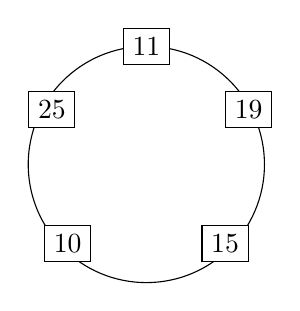
\begin{tikzpicture}[x=1.0cm,y=1.0cm, fill=white]
\draw(2,2) circle (1.5cm);
\draw (2,3.5) node[fill=white,draw] {11};
\draw (3.3,2.7) node[fill=white,draw] {19};
\draw (0.8,2.7) node[fill=white,draw] {25};
\draw (1,1) node[fill=white,draw] {10};
\draw (3,1) node[fill=white,draw] {15};
\end{tikzpicture}
\end{center}

\noindent 
 A cél a minimális számú gyufaszál átrakása. Hogyan lehet elérni?

\end{enumerate}

\subsection*{2006.04.12.}
\begin{enumerate}
\item $[x]$ jelöli azt a legnagyobb egész számot, ami nem nagyobb $x$-nél.\\ Például: 
$[2,1]=2$\quad $[-0,2]=-1$ \quad $[3]=3$\quad$0,2]=1$\quad
$[-1,3]=-2$\\
Ábrázoljuk az $x \mapsto [x]$ függvényt!
\item 
\begin{abc}
\item $x \mapsto [x]-1$;
\item $x \mapsto [x-1]$;
\item $x \mapsto 2[x]$;
\item $x \mapsto [2x]$;
\item $x \mapsto [-x]$;
\item $x \mapsto -[x]$.
\end{abc}
\end{enumerate}

\subsection*{2006.04.19.}
Ábrázoljuk a következő függvényeket:
\begin{enumerate}
\item $x \mapsto |[x]|$;
\item $x \mapsto [|x|]$;
\item $x \mapsto [x-1]$;
\item $x \mapsto [x]-1$;
\item $x \mapsto [-x]$;
\item $x \mapsto -[x]$;
\item $x \mapsto x-[x]$;
\item $x \mapsto [2x-1]$;
\item $x \mapsto 3[x]+1$;
\item $x \mapsto [x]+[-x]$.
\end{enumerate}

\subsection*{2006.04.25.}
Ábrázoljuk a következő függvényeket:
\begin{enumerate}
\item $x \mapsto x^2-1$;
\item $x \mapsto (x-1)^2$;
\item $x \mapsto -x^2$;
\item $x \mapsto -(x-1)^2$;
\item $x \mapsto [x]^2$;
\item $x \mapsto [x^2]$;
\item $x \mapsto x|x|$;
\item $x \mapsto x[x]$;
\item $x \mapsto x^2-4x+5$;
\item $x \mapsto x^2-6x+7$;
\end{enumerate}

\subsection*{2006.04.26.}
Ábrázoljuk a következő függvényeket:
\begin{enumerate}
\item $x \mapsto x^2-2x$;
\item $x \mapsto x^2-2|x|$;
\item $x \mapsto |x^2-2x|$;
\item $x \mapsto |x^2-2|x||$;
\item $x \mapsto |x^-1|$;
\item $x \mapsto x^2-4x$;
\item $x \mapsto x^2-4|x|$;
\item $x \mapsto 4|x|-x^2$;
\item $x \mapsto 4x^2-4|x|$;
\item Hol vannak a síkon azok a $P(x;y)$ pontok amelyekre teljesül, hogy $|x|+|y|\le5$?
\end{enumerate}

\subsection*{2006.04.27.}
\begin{enumerate}
\item Hol vannak a síkon azok a $P(x;y)$ koordinátájú pontok, amelyekre teljesül:
\begin{abc}
\item $|x+y|\le2$;
\item $|x-y|\le2$;
\item $y\le2x+1$ és $y\ge2x-2$.
\end{abc}
\item Ábrázoljuk a következő függvényeket:
\begin{abc}
\item $x \mapsto 2x^2$;
\item $x \mapsto 2(x-1)^2+1$;
\item $x \mapsto 2x^2+4x$;
\item $x \mapsto 2x^2+4|x|$;
\item $x \mapsto -2x^2+4|x|$.
\end{abc}
\end{enumerate}

\subsection*{2006.05.02.}
\begin{enumerate}
\item Hol vannak a síkon azok a $P(x;y)$ pontok, amelyekre teljesül:
\begin{abc}
\item $x^2-4\le y \le-x^2+4$;
\item $-x^2\le y \le x^2$;
\item $2x^2-4|x|\le y \le -2x^2+4|x|$.
\end{abc}
\item Oldjuk meg a következő egyenlőtlenségeket:
\begin{abc}
\item $x^2-4x \le 0$;
\item $x^2-4|x| \le 0$;
\item $4|x|-2x^2 \ge 0$;
\item $6|x|-x^2 \ge 0$.
\end{abc}
\end{enumerate}

\subsection*{2006.05.03.}
\begin{enumerate}
\item Ábrázoljuk a következő függvényeket:
\begin{abc}
\item $x \mapsto \frac{1}{x-1}, x\neq1$;
\item $x \mapsto \frac{1}{x+2}, x\neq-2$;
\item $x \mapsto \frac{x-3}{x-2}, x\neq2$;
\item $x \mapsto \frac{1}{|x|}, x\neq0$;
\item $x \mapsto \left|\frac{x-2}{x-1}\right|, x\neq1$;
\item $(*)$ $ x \mapsto \left[\frac{1}{x}\right], x\neq0$;
\item $x \mapsto \frac{1}{[x]}, x\ge 1, x<0$.
\end{abc}
\end{enumerate}

\subsection*{2006.05.16.}
\begin{enumerate}
\item Ábrázoljuk a következő függvényeket:
\begin{abc}
\item $x \mapsto |x^2-4|x|+3|$;
\item $x \mapsto \left|\frac{|x|-2}{|x|-1}\right|, |x|\neq1$;
\item $x \mapsto \left|\frac{x^2-6|x|+9}{|x|-3}\right|, |x|\neq3$;
\item $x \mapsto \left|\frac{|x|-3}{|x|-2}\right|, |x|\neq2$.
\end{abc}
Oldjuk meg függvények segítségével a következő egyenlőtlenségeket:
\begin{abc}
\item $x \mapsto -|x|+3\le y \le |x|-3$;
\item $x \mapsto x^2-4 \le y \le -x^2+4$;
\item $(*)$ $x \mapsto x^2-4x \le y \le 2x+5$.
\end{abc}
\end{enumerate}

\subsection*{2006.05.17.}
Ábrázoljuk a következő függvényeket:
\begin{enumerate}
\item $x \mapsto [-2x+3]$;
\item $x \mapsto |x^2-4|x||$;
\item $x \mapsto \left|\frac{|x|-1}{|x|-2}\right|, |x|\neq2$;
\item $x \mapsto \left[\frac{1}{x-1}\right], x\neq1$.
\end{enumerate}
Oldjuk meg a következő egyenlőtlenségeket:
\begin{enumerate}
\item $x^2-2x-3 \le 0$;
\item $1-\frac{1}{x-1}>0$;
\item $|x|-2 \le y \le 4-x$?
\end{enumerate}

\section{Halmazok}

\subsection*{2006.05.23.}
\begin{enumerate}
\item Sorold fel a következő halmaz összes részhalmazát:
(a) $\{1, 2, 3\}$;  (b) $\{1, 2, 3, 4\}$.
\item Adjuk meg az $A\cap B$, $A\cup B$, $A\setminus B$, $B\setminus A$ halmazokat, ha
\begin{abc}
\item $A = \{-1, 0, 3, 4\}$, $B=\{0, 4, 6\}$;
\item $A = \{0,1,2,3\}$, $B=\{-1,0,1,2,3\}$;
\item $A = [0; 2]$, $B = [1;3]$.
\end{abc}
\item Igazoljuk, hogy tetszőleges $A, B, C$ halmazokra teljesülnek a következő azonosságok:
\begin{abc2}
\item $A\cup(A\cap B)=A$;
\item $A\cap(A\cup B)=A$;
\item $((A\setminus B)\setminus C)=(A\setminus C)\setminus B$;
\item $A\setminus(A\setminus B) = A\cap B$;
\item $A\setminus(B\cap C)=(A\setminus B)\cup(A\setminus C)$.
\end{abc2}
\end{enumerate}
\subsection*{2006.05.25.}
\begin{enumerate}
\item $A=\{2,4,6,8,10\}$, $B=\{3,6,9,12,15\}$ és $C=\{5,10,15,20\}$.
\begin{abcn}{5}
\item $A\cup B\cup C=?$
\item $A\cap B\cap C=?$
\item $A\setminus B=?$
\item $C\setminus A=?$
\item $B\setminus C=?$
\end{abcn}
\item Melyek azok az $A$ és $B$ halmazok, amelyekre teljesül a következő három egyenlőség:
\begin{abc}
\item $A\cap B=\{3,5,7\}$, $A\setminus B=\{2,6\}$, $A\cup B=\{1,2,3,4,5,6,7\}$;
\item $A\setminus B=\{1,2,5\}$, $B\setminus A=\{7,8,9\}$, $A\cap B=\{3,4,6\}$.
\end{abc}
\item Az $A$ halmaznak 8, a $B$-nek 9 eleme van, $A\cup B$-nek 15 eleme van. Hány eleme van $A\cap B$-nek?
\item Írjuk fel a következő halmazokat elemeik felsorolásával:
\begin{abc2}
\item $A=\{x\in \mathbb{N} ~|~ \frac{24}{x}\in \mathbb{Z}\}$
\item $B=\{x\in \mathbb{Z} ~|~ -5\le x \le 4\}$
\item $C=\{x\in \mathbb{Z} ~|~ |x-3|=5\}$
\item $D=\{x\in \mathbb{Q} ~|~ |x-3|+|x-1|=3\}$
\end{abc2}
\item Az $\mathbb{N}$ halmazt részhalmazokra bontottuk:
$\{0\}, \{1,2\}, \{3,4,5\}, \{6,7,8,9\}, \ldots$
Melyik számmal kezdődik a századik részhalmaz?
\end{enumerate}

\subsection*{2006.05.30.}
\begin{enumerate}
\item $A$: a páros kétjegyű számok halmaza; $B$: a 100-nál kisebb, 3-mal osztható számok halmaza; $C$: a 30-cal osztható egész számok halmaza.
$
A\cap B=?\qquad
A\cap C=?\qquad
B\cap C=?
$
\item Adjunk példát olyan $A$, $B$ és $C$ halmazra, hogy teljesüljenek:
$|A\cap B \cap C|=1$, $|A|=|B|=|C|=2$ és $A\ne B$, $B\ne C$.
\item $A=B=\{0,1,2\}$, $A\times B=?$
\item Tudjuk, hogy $A\cup B=\{1,2,3,4,5,6\}$, $A\setminus B=\{2,4,6\}$, 
$A\cap B=\{1,3\}$. $A=?$, $B=?$
\item ($*$) Tudjuk, hogy $|A \times B|=100$. Mekkora lehet $|A\cup B|$ legalább és legfeljebb?
\item $A=\{1,2,3\}$, $B=\{2,3,4\}$. Hány eleme van a következő halmazoknak?
\begin{abc4}
\item $(A\setminus B)\times(B\setminus A)$;
\item $(A\cup B)\times(A\cap B)$;
\item $(A\setminus B)\times(A\cap B)$;
\item $(B\setminus A)\times(B\cup A)$.
\end{abc4}
\item Tudjuk, hogy $|A|=5$, $|B|=8$, $|A\setminus B|=3$. $|A\cap B|=?$, $|A\cup B|=?$
\end{enumerate}

\subsection*{2006.05.31.}
\begin{enumerate}
\item Legyen $A=\{\text{a 7-tel osztható kétjegyű számok}\}$,
$B=\{\text{a 3-mal osztható kétjegyű számok}\}$. $|A\cup B|=?$, $|A\cap B|=?$
\item Hány eleme van legalább annak a halmaznak, amelynek legalább 1000-rel több részhalmaza van, mint eleme?
\item Egy 15 elemű halmaznak 9 elemű részhalmazából vagy a 6 elemű részhalmazából van több?
\item Hány háromelemű részhalmaza van az $\{1,2,3,4,5\}$ halmaznak?
\item Legyen $A$ az 1000-nél kisebb pozitív egész számok halmaza. Hány elemű $A$ összes részhalmazának egyesítése?
\item $A=\{1,2\}$, $B=\{1,2,3,4\}$. $(A\times A)\cap(B\times B)=?$
\item Hány olyan részhalmaza van az egyjegyű pozitív egész számok halmazának, amelynek
\begin{abc3}
\item a 4 és az 5 is eleme;
\item a 4 eleme, de az 5 nem;
\item sem az 5, sem a 4 nem eleme?
\end{abc3}
\item Hány olyan részhalmazát lehet megadni az $A$ halmaznak, hogy semelyik kettő közös része se legyen üres, ha
(a) $A=\{1,2,3,4\}$;\quad (b) $A=\{1,2,3,4,5,6,7,8\}$?
\end{enumerate}

\subsection*{2006.06.01.}

\begin{enumerate}
\item $A\cup B=\{1,2,3,4,5\}$, $A\cap B=\{3,5\}$, $A\setminus B=\{1\}$,
$B\setminus A=\{2,4\}$. $A=?$, $B=?$
\item $A\cup B=\{1,2,3,4,5\}$, $A\setminus B=\{1,4\}$, $A\cap B\not\subset\{3,4,5\}$, $|A|=|B|$. $A=?$, $B=?$
\item Hány páros számú elemet tartalmazó részhalmaza van az $A=\{1,2,3,4,5\}$ halmaznak? És hány páratlan számú elemet tartalmazó részhalmaza van?
\item ($*$) Legyen $M=\{\frac{2}{1},\frac{4}{3},\frac{6}{5},\frac{8}{7},\ldots,\frac{1002}{1001}\}$. Hány olyan $x$ eleme van az $M$ halmaznak, amelyekre $|x-1|<0{,}1$?
\item Legyenek $A$, $B$ és $C$ olyan halmazok, amelyekre $A\cap C = B\cap C$ és
$A\setminus C=B\setminus C$. Igazoljuk, hogy ekkor $A=B$.
\item ($*$) Mutass példát három olyan halmazra, hogy bármely kettőnek végtelen sok közös eleme van, de a három halmaz közös része üres.
\item Legyen $A=\{x\in \mathbb{R}~|~x|\le 1\}$, $B=\{y\in \mathbb{R}~|~|y|\le 1\}$.
Milyen ponthalmazt határoznak meg azok az $(x;y)$ koordinátapárok, amelyek az $A\times B$ halmaz elemeit alkotják?
\end{enumerate}

\subsection*{Témazáró -- 2006.06.06.}

\begin{enumerate}
\item Írjuk fel külön-külön sorba az $A=\{1,3,5,7\}$ halmaz 0; 1; 2; 3; 4; elemű részhalmazait!
\item Adjunk meg három olyan kételemű halmazt, melyeknek páronként vett közös része nem üres halmaz, de mindhárom halmaznak nincs közös eleme.
\item Az $A$, $B$, $C$ halmazok mindegyikének 5 eleme van, $|A\cap B \cap C|=1$.
Mekkora lehet $A\cup B \cup C$ maximális és minimális elemszáma?
\item Legyen $A=\{x\in\mathbb{N} ~|~ 2x\le 4x-6\}$ és $B=\{x\in\mathbb{N}~|~4x-11\le 2x+11\}$. Mik az elemei az $A\cap B$ halmaznak?
\item Hány eleme van annak a $P(x;y)$ pontokból halmaznak, amelyre teljesül, hogy $|x|+|y|\le 5$ és $x,y$ egész számok? Ábrázold a halmazt!
\item A $H$ halmaz a következő:
$$H=\left\{\frac{2}{3},\frac{4}{5},\frac{6}{7},\ldots,\frac{400}{401}\right\}.$$
Hány olyan $x$ eleme van $H$-nak, amelyre igaz, hogy $|x-1|<\frac{1}{100}$?
\end{enumerate}



\chapter{C05, 9. évfolyam}
\section{Sorozatok}

\subsection*{2007. 09. 05. -- Sorozatok}
\begin{enumerate}
\item Legyen  $a_n=1+2+\ldots+n$, írjuk fel $a_{10}$, $a_{100}$ és $a_{200}$ értékét!
\item Adott két sorozat: $a_n=n^2+3$, $b_n=n^2-2$.  Hány közös eleme van a két sorozatnak?
\item Legyen $a_n$ a $2^n$ szám tízes számrendszerbeli alakjának utolsó két jegye. $a_{100}=\,?$
\item Egy $a_n$ sorozat mindegyik eleme a másodiktól kezdve a szomszédos elemek számtani közepe;
$a_1=1$, $a_5=9$. Írjuk fel a sorozat első 10 elemét!
\item Igaz-e, hogy az $a_n=n^2+3n-2$ sorozat elemei között végtelen sok összetett szám van?
\item Egy sorozat definíciója: $a_1=a$, $a_2=b$ és $\displaystyle{a_{n+1}=\frac{a_n+a_{n+2}}{2}}$ ha $n\ge 1$.
Mutassuk meg, hogy a sorozat szomszédos tagjainak különbsége állandó!
\end{enumerate}


\subsection*{2007. 09. 09. --  Számtani sorozatok}
\begin{enumerate}
\item Írjuk fel a következő \textit{számtani sorozatok} tizedik tagját!
\begin{abc}
\item $2, 4, 6, 8, \ldots$
\item $\frac{1}{3}, \frac{1}{12}, -\frac{1}{6},\ldots$
\item $a-b, b, 3b-a, \ldots$
\item $a^2, 1, 2-a^2,\ldots$
\end{abc}

\item Határozzuk meg az $a$ paraméter értékét, ha a következő három szám egy számtani sorozat első három eleme:
\begin{abcn}{6}
\item $1, 3, a$;
\item $1, a, 3$;
\item $a-1, 3, a+1$;
\item $a, a^2, 0$;
\item $a, a^2, a^3$;
\item $a^2, a, a^3$.
\end{abcn}

\item Egy számtani sorozat első két tagjának összege 7, harmadik és negyedik tagjának összege 19. Írjuk fel a sorozat első négy tagját!

\item ($*$) Bizonyítsuk be, hogy nincs olyan számtani sorozat, amelynek tagjai között a
$\sqrt 2$, $\sqrt 3$ és $\sqrt 5$ is szerepel!

\item Határozzuk meg a 101 és 501 közé eső olyan egészek összegét, amelyek
\begin{abc}
\item oszthatók 5-tel;
\item oszthatók 3-mal;
\item 12-vel osztva 7 maradékot adnak!
\end{abc}
\end{enumerate}


\subsection*{2007. 09. 11.}
\begin{enumerate}
\item Egy csökkenő számtani sorozat első 17 tagjának összege 0. Hány pozitív tagja van a sorozatnak?
\item Négy pozitív szám egy számtani sorozat négy szomszédos tagja, összegük 26, szorzatuk 880.
Melyek ezek a számok? 
\item Egy $(a_n)$ sorozatról tudjuk, hogy tetszőleges $k$ pozitív egész esetén $a_1+a_2+a_3+\ldots+a_k=k^2$. Bizonyítsuk be, hogy $(a_n)$ számtani sorozat! $a_{100}=\,?$
\item Mi az első három eleme annak a számtani sorozatnak, amelyre az első $n$ tag összege minden $n$ esetén
\begin{abc3}
\item $n^2+n$;
\item $n^2-n$;
\item $5n^2-3n$?
\end{abc3}
\item Határozzuk meg annak a számtani sorozatnak az első tagját,
amelyben az első három tag összege negyed\-része a következő három tag összegének. 
\item Bizonyítsuk be, hogy ha $x$, $y$, $z$ számok egy számtani sorozat szomszédos elemei,
akkor $x^2+xy+y^2$, $x^2+xz+z^2$ és  $y^2+yz+z^2$ is egy számtani sorozat szomszédos elemei.
\end{enumerate}


\subsection*{2007. 09. 12. -- Röpdolgozat}
\begin{enumerate}
\item 4 és 40 közé írjunk be három számot úgy, hogy a kapott öt szám egy számtani sorozat első öt eleme legyen.
\item Egy növekvő számtani sorozat első három tagjának összege 27, ugyanezen tagok négyzetét összeadva 275-öt kapunk. Melyik ez a sorozat?
\end{enumerate}

\subsection*{2007. 09. 17. -- Röpdolgozat}
\begin{enumerate}
\item Bizonyítsuk be, hogy ha $a^2$, $b^2$ és $c^2$ egy számtani sorozat egymást követő elemei, 
akkor $\displaystyle{\frac{1}{b+c}}$, 
$\displaystyle{\frac{1}{c+a}}$ és
$\displaystyle{\frac{1}{a+b}}$ is egy számtani sorozat egymást követő elemei.
\item Egy számtani sorozat három egymást követő elemének összege 3, köbeik összege 15. Írjuk fel a sorozat ötödik elemét!
\end{enumerate}

\subsection*{2007. 09. 18.}
\begin{enumerate}
\item Határozzuk meg a mértani sorozat első három elemét, ha
\begin{abc3}
\item $a_8=2^8$ és $q=-2$;
\item $a_8=0{,}1$ és $q=0{,}1$;
\item $a_{10}=x^{20}$ és $q=\sqrt[3]{x}$.
\end{abc3}
\item Mi a mértani sorozat ötödik tagja, ha 
\begin{abc3}
\item $a_2=a_1^2$ és $\displaystyle{q=-\frac{8}{a_1^2}}$;
\item $a_1a_2=a_1+a_2$ és $a_3=3q$;
\item $a_3=2$ és $a_6=\displaystyle{\frac{1}{4}}$?
\end{abc3}
\item Határozzuk meg a mértani sorozat első tagját és hányadosát, ha tudjuk, hogy 
\begin{abc2}
\item $a_1+a_2=6$ és $a_4+a_3=24$;
\item $a_1+a_2+a_3=42$ és $a_1a_3=64$.
\end{abc2}
\item Mennyi a mértani sorozat első öt tagjának összege, ha
\begin{abc4}
\item $a_1=2$ és $q=3$;
\item $a_2=a$ és $\displaystyle{a_4=\frac 1a}$;
\item $a_4=10$ és $q=3$;
\item $a_{10}=1$ és $\displaystyle{a_{20}=\frac{1}{22}}$.
\end{abc4}
\end{enumerate}

\subsection*{2007. 09. 19. -- Röpdolgozat}
\begin{enumerate}
\item Egy mértani sorozat első 10 tagjának összege 30, első 20 tagjának összege 60.
Mi a sorozat első eleme és hányadosa?
\item Egy számtani sorozat három szomszédos tagjának összege 21. Ha a három taghoz rendre
3-at, 1-et és 3-at adunk, akkor egy mértani sorozat szomszédos tagjait kapjuk. Mennyi a mértani sorozat 
hányadosa?
\end{enumerate}

\subsection*{2007. 09. 19.}
\begin{enumerate}
\item Egy mértani sorozatban $S_3=1$ és $S_4=3S_2$. Mi a mértani sorozat első három tagja?
\item Egy derékszögű háromszög oldalainak mérőszámai egy mértani sorozat szomszédos elemei. Adjuk meg a sorozat hányadosát!
\item Egy mértani sorozat első három tagjának összege 52. Ha az első taghoz 2-t, a másodikhoz 10-et, a harmadikhoz 2-t adunk, akkor egy számtani sorozat szomszédos elemeit kapjuk. Mi a mértani sorozat első eleme és hányadosa?
\item Három szám egy mértani sorozat három egymás utáni tagja. Ha a másodikhoz 8-at adunk, akkor egy számtani sorozat egymás utáni elemeit kapjuk. Ha ennek a számtani sorozatnak a harmadik eleméhez 64-et adunk, akkor egy új mértani sorozat három egymást követő elemét kapjuk. Melyik ez a három szám?
\end{enumerate}

\subsection*{2007. 09. 24. -- Röpdolgozat}
\begin{enumerate}
\item Egy növekvő mértani sorozatban az első négy tag összege 30, a második négy tag összege 480. Mennyi a sorozat 
első tagja és hányadosa?
\item Négy szám közül az első három egy számtani sorozat három egymást követő eleme, az utolsó három pedig egy mértani sorozat
három egymás utáni eleme. A két szélső összege 14, a két középső szám összege 12. Melyik ez a négy szám?
\end{enumerate}

\subsection*{2007. 09. 25. -- Röpdolgozat}
\begin{enumerate}
\item Négy szám egy mértani sorozat első négy eleme. Az első és a negyedik szám összege 112, a második és harmadik szám összege 48. Mi a mértani sorozat első tagja és hányadosa?
\item Egy mértani sorozat első három tagjának összege 26. Ha a három taghoz sorra 1-et, 6-ot és 3-at adunk, akkor egy számtani
sorozat három egymást követő tagját kapjuk. Melyik ez a három szám?
\end{enumerate}

\subsection*{2007. 10. 01.}
\begin{enumerate}
\item Számítsuk ki az alábbi összegeket:
\begin{abc2}
\item $\displaystyle{1+11+111+\ldots+\underbrace{111\ldots 1}_{n}}$;
\item $\displaystyle{3+2\cdot 3^2+\ldots+n\cdot 3^n}$.
\end{abc2}
\item Számítsuk ki az alábbi összegeket:
\begin{abc}
\item $\displaystyle{\frac{1}{1\cdot 2}+\frac{1}{2\cdot 3}+\frac{1}{3\cdot 4}+\ldots+\frac{1}{(n-1)n} }$;
\item $\displaystyle{\frac{1}{1\cdot 2\cdot 3}+\frac{1}{2\cdot 3\cdot 4}+\frac{1}{3\cdot 4\cdot 5}+\ldots+\frac{1}{(n-2)(n-1)n} }$;
\item $\displaystyle{1\cdot 2+2\cdot 3+3\cdot 4+\ldots+n(n+1)}$;
\item $\displaystyle{1\cdot 2\cdot 3+2\cdot 3\cdot 4+3\cdot 4\cdot 5+\ldots+n(n+1)(n+2)}$.
\end{abc}
\item Egy számtani sorozatról tudjuk, hogy a negyedik tagja 4.
A sorozat $d$ különbségének mely értékeire igaz, hogy a sorozat első három tagjának páronként vett szorzatát összeadva a legkisebb értéket kapjuk?
\end{enumerate}

\subsection*{2007. 10. 02. -- Röpdolgozat}
\begin{enumerate}
\item  Számítsuk ki a következő összeget:
$$\frac{1}{1\cdot 3}+\frac{1}{3\cdot 5}+\frac{1}{5\cdot 7}+ \ldots+\frac{1}{(2n-1)(2n+1)}=\,?$$
\item Adjuk meg zárt alakban a következő összeget:
$$1+3x+5x^2+\ldots+(2n-1)x^{n-1}=\,?$$
\end{enumerate}

\subsection*{2007. 10. 03. -- Újabb röpdolgozat}
\begin{enumerate}
\item Egy mértani sorozat első három elemének összege 93. E három elem egyúttal egy számtani sorozat első, második illetve hetedik eleme. Adjuk meg ezeket a sorozatokat! 
\item Adjuk meg zárt alakban a következő összeget:
$$\left(x+\frac{1}{x}\right)^2+\left(x^2+\frac{1}{x^2}\right)^2+\ldots+\left(x^n+\frac{1}{x^n}\right)^2 .$$
\end{enumerate}

\subsection*{2007. 10. 03.}
\begin{enumerate}
\item Egy számtani sorozatról tudjuk, hogy a negyedik tagja 4.
A sorozat $d$ különbségének mely értékeire igaz, hogy a sorozat első három tagjának páronként vett szorzatát összeadva a legkisebb értéket kapjuk?
\item Három számjegy egy mértani sorozat első három tagja. A számok átlaga $\frac{14}{3}$, szorzata 64. Melyik ez a sorozat?
\item Egy háromjegyű szám számjegyei egy mértani sorozat első három tagja, a 400-zal kisebb szám számjegyei egy számtani sorozat első három tagja. Melyik ez a szám?
\item Az $5x-y$, $2x+3y$ és $x+2y$ egy számtani sorozat első három tagja,
az $(y+1)^2$, $xy+1$ és $(x-1)^2$ számok pedig egy mértani sorozat első három tagja. $x=\,?$, $y=\,?$
\end{enumerate}

\subsection*{2007. 10. 08.}
\begin{enumerate}
\item Számítsuk ki (adjuk meg zárt alakban):
\begin{abc}
\item $\displaystyle{1+2+3+\ldots+n=\sum_{k=1}^n k = \frac{n(n+1)}{2}}$
\item $\displaystyle{1^2+2^2+3^2+\ldots+n^2=\sum_{k=1}^n k^2 =}$
\item $\displaystyle{1^3+2^3+3^3+\ldots+n^3=\sum_{k=1}^n k^3 =}$
\item $\displaystyle{1^4+2^4+3^4+\ldots+n^4=\sum_{k=1}^n k^4 =}$
\end{abc}
\item Számítsuk ki:
\begin{abc3}
\item $\displaystyle{\sum_{k=1}^n k(k+1)}$;
\item $\displaystyle{\sum_{k=1}^n k(k+1)(k+2)}$;
\item $\displaystyle{\sum_{k=1}^n k(k+1)(k+2)(k+3)}$. 
\end{abc3}
\item Számítsuk ki: 
\begin{abc3}
\item $\displaystyle{\sum_{k=1}^n \frac{1}{k(k+1)}}$;
\item $\displaystyle{\sum_{k=1}^n \frac{1}{k(k+1)(k+2)}}$;
\item $\displaystyle{\sum_{k=1}^n \frac{1}{k(k+1)(k+2)(k+3)}}$.
\end{abc3}
\end{enumerate}

\subsection*{2007. 10. 10.}
\begin{enumerate}
\item Igazoljuk, hogy 
$$1\cdot 2\cdot 3\cdot\ldots\cdot k+
2\cdot 3\cdot\ldots\cdot k(k+1)+\ldots+
n(n+1)\ldots(n+k-1)=\frac{n(n+1)\ldots(n+k)}{k+1}.$$ 
\item Számítsuk ki:
\begin{abc}
\item $\displaystyle{1^3+3^3+5^3+\ldots+(2n-1)^3}$;
\item $\displaystyle{1\cdot 1!+2\cdot 2!+3\cdot 3!+\ldots+n\cdot n!}$; 
\item $\displaystyle{\left(1+\frac{1}{3}\right)
\left(1+\frac{1}{9}\right)\left(1+\frac{1}{81}\right)\ldots\left(1+\frac{1}{3^{2n}}\right)
}$.
\end{abc}
\item Számítsuk ki:
$$\binom{n+1}{1}+\binom{n+2}{2}+\binom{n+3}{3}+\ldots+\binom{n+k}{k}.$$
\item ($*$) Igazoljuk a következő egyenlőtlenségeket:
\begin{abc}
\item $\displaystyle{\left(1+\frac{1}{n}\right)^n < 
\left(1+\frac{1}{n+1}\right)^{n+1}}$; 
\item $\displaystyle{
\left(1+\frac{1}{n}\right)^{n+1} > 
\left(1+\frac{1}{n+1}\right)^{n+2}
}$, ahol $n>0$ egész szám.
\end{abc}
\end{enumerate}

\subsection*{2007. 10. 12. -- Ismétlő feladatok}
\begin{enumerate}
\item Vizsgáljuk meg a következő sorozatokat növekedés-fogyás szempontjából:
\begin{abc}
\item $\displaystyle{a_1=1,\qquad a_{n+1}=\frac{1}{1+a_n}}$;
\item $\displaystyle{a_1=4,\qquad a_{n+1}=\frac{2+a_n^2}{2a_n}}$.
\end{abc}
\item Legyen $a_1=2$, $a_2=1$, $a_{n+2}=\frac{a_n+a_{n+1}}{2}$. Fejezzük ki $a_n$-et $n$-nel!
\item Az $1, 4, 10, 19,\ldots$ sorozat szomszédos tagjainak különbségsorozata számtani sorozat. Adjuk meg a sorozat $n$-edik tagját és első $n$ tagjának összegét.
\item Adott a következő táblázat:

$1$

$2, 3, 4$

$3, 4, 5, 6, 7$

$4, 5, 6, 7, 8, 9, 10$

\noindent Igazoljuk, hogy a sorok összege mindig négyzetszám!
\end{enumerate}

\subsection*{2007. 10. 15. -- A Fibonacci-sorozat tulajdonságai}
\begin{enumerate}
\item $f_1=f_2=1$, $f_{n+2}=f_n+f_{n+1}$.
\begin{abc}
\item $\displaystyle{f_1+f_3+f_5+\ldots+f_{2n-1}}=\,?$
\item $\displaystyle{f_2+f_4+f_6+\ldots+f_{2n}}=\,?$
\item $\displaystyle{f_{n+1}f_{n-1}-f_n^2}=\,?$
\item $\displaystyle{f_1^2+f_2^2+f_3^2+\ldots+f_n^2}=\,?$
\end{abc}
\item 
\begin{abc}
\item $\displaystyle{f_1^2+f_2^2+f_3^2+\ldots+f_n^2}=\,?$
\item $\displaystyle{f_1+f_2+f_3+\ldots+f_n}=\,?$
\item $\displaystyle{\binom{2n}{0}+\binom{2n-1}{1}+\binom{2n-2}{2}+\ldots+\binom{n}{n}}=\,?$
\item $\displaystyle{\binom{2n-1}{0}+\binom{2n-2}{1}+\binom{2n-3}{2}+\ldots+\binom{n}{n-1}}=\,?$
\end{abc}
\item Igazoljuk, hogy bármely két szomszédos Fibonacci-szám legnagyobb közös osztója 1.
\item Melyek azok a Fibonacci-számok, amelyek oszthatók \textit{a}) 3-mal; \textit{b}) 5-tel?
\end{enumerate}

\subsection*{2007. 10. 17.}
\begin{enumerate}
\item Igazoljuk a következő egyenlőtlenségeket:
\begin{abc}
\item $\displaystyle{\left(1+\frac{2}{n}\right)^n < 
\left(1+\frac{2}{n+1}\right)^{n+1}}$, ha $n>0$ egész; 
\item $\displaystyle{\left(1-\frac{1}{n}\right)^n < 
\left(1-\frac{1}{n+1}\right)^{n+1}
}$.
\end{abc}
\item Igazoljuk, hogy ha $n \ge 1$ egész, akkor
$$0<\left(1+\frac{1}{n}\right)^{n+1}-
\left(1+\frac{1}{n}\right)^n<\frac{4}{n}.$$
\item ($*$) Igazoljuk, hogy ha $n \ge 1$ egész, akkor
$$\frac{1\cdot 3\cdot \ldots \cdot (2n-1)}{2\cdot 4\cdot \ldots \cdot 2n} < \frac{1}{\sqrt{2n+1}}.$$
\item  Bizonyítsuk be, hogy ha $n \ge 3$ egész, 
akkor $n^{n+1} > (n+1)^n$. 
\item Mutassuk meg, hogy ha $n \ge 2$ egész, akkor
$$1+\frac{1}{\sqrt{2}}+\frac{1}{\sqrt{3}}+
\ldots+\frac{1}{\sqrt{n}} > \sqrt{n}.$$
\item Igazoljuk, 
hogy $\left(2n\right)!
<2^{2n}\cdot \left(n!\right)^2$, ha $n > 0$ egész.
\end{enumerate}

\subsection*{2007. 10. 27.}
\begin{enumerate}
\item Igazoljuk, hogy négyzetszám:
\begin{abc3}
\item $\displaystyle{\underbrace{44\ldots 4}_{n+1}
\underbrace{88\ldots 8}_{n}9}$; \qquad
\item $\displaystyle{\underbrace{11\ldots 1}_{n}
\underbrace{22\ldots 2}_{n} - \underbrace{33\ldots 3}_{n}}$; \qquad
\item $\displaystyle{\underbrace{44\ldots 4}_{n+1}
\underbrace{88\ldots 8}_{n}9}$.
\end{abc3}
\item ($*$) Igazoljuk, hogy a következő számok között végtelen sok négyzetszám van:
$$1, \quad 
1+2, \quad
1+2+3, \quad
1+2+3+4, \quad
\ldots, \quad
1+2+3+\ldots+n, \quad
\ldots $$
\item Számítsuk ki az alábbi összeget:
$$nx+(n-1)x^2+\ldots+2x^{n-1}+x^n.$$
\item Igazoljuk, hogy a következő sorozatok növekednek, de felülről korlátosak:
\begin{abc2}
\item $a_1=\sqrt 2$, \quad $a_{n+1}=\sqrt{2+a_n}$; \qquad
\item $a_1=\sqrt 5$, \quad $a_{n+1}=\sqrt{5+a_n}$.
\end{abc2}
\end{enumerate}

\subsection*{2007. 11. 07. -- Sorozatok (dolgozat)}
\begin{enumerate}
\item Egy számtani sorozatban $a_3=5$ és $a_5=3$. 
Határozzuk meg $a_n$ és $S_n$ értékét!
\item Számítsuk ki a következő összeget:
$$2\cdot 1^2+3\cdot 2^2+4\cdot 3^2+\ldots+(n+1)n^2.$$
\item Egy sorozatban $a_1=1$ és $a_{n+1}=2a_n+1$, ha $n \ge 1$.
Számítsuk ki $a_1+a_2+a_3+\ldots+a_n$ értékét.
\item Egy mértani sorozat első három elemének összege 93. Ez a három elem egyúttal egy számtani sorozat első, második és hetedik eleme. Adjuk meg a sorozatokat.
\item Számítsuk ki a következő összeget:
$$\frac{1^2}{1\cdot 3}+ 
\frac{2^2}{3\cdot 5}+
\frac{3^2}{5\cdot 7}+\ldots+
\frac{n^2}{(2n-1)(2n+1)}.$$
\end{enumerate}


\section{Trigonometria}

\subsection*{2007. 11. 19. -- Trigonometria}
%ru3022
%KL/AM
\begin{enumerate}
\item Ábrázoljuk a következő függvényeket:
\begin{abc4}
\item $x \mapsto \sin 2x$;
\item $x \mapsto \sin \frac{1}{2}x$;
\item $x \mapsto |\sin x|$;
\item $x \mapsto \sin |x|$.
\end{abc4}
\item Igazoljuk, hogy
\begin{abc}
\item $\displaystyle{\frac{1}{\cos^2\alpha}=\tg^2\alpha+1}$, ha $\displaystyle{\alpha \ne \frac{\pi}{2}+n\pi}$, $\alpha \in \mathbb{Z}$;
\item $\displaystyle{\frac{1}{\sin^2\alpha}=\ctg^2\alpha+1}$, ha $\alpha \ne n\pi$, $n \in \mathbb{Z}$.
\end{abc}
\item Ábrázoljuk:
\begin{abc}
\item $x \mapsto \tg 2x$; \qquad $\displaystyle{x \ne \frac{\pi}{4}+k\frac{\pi}{2}}$, $k \in \mathbb{Z}$;
\item $x \mapsto \tg |x|$;  \qquad $\displaystyle{x \ne \frac{\pi}{2}+n\pi}$, $n \in \mathbb{Z}$;
\item $x \mapsto \ctg \frac{1}{2}x$; \qquad $\displaystyle{x \ne 2n\pi}$, $n \in \mathbb{Z}$.
\end{abc}
\item Oldjuk meg a kövekező egyenleteket:
\begin{abc4}
\item $\displaystyle{\sin x=\frac{1}{2}}$;
\item $\displaystyle{\cos x=\frac{\sqrt{3}}{2}}$;
\item $\displaystyle{\tg x=1}$;
\item $\displaystyle{\ctg x=\sqrt{3}}$.
\end{abc4}
\end{enumerate}

\subsection*{2007. 11. 20. -- Trigonometriai azonosságok}
%ru3023
%KL
\begin{enumerate}
\item Igazoljuk a következő azonosságokat:
\begin{abc}
\item $\sin(\alpha \pm \beta)=\sin\alpha \cos\beta \pm \cos\alpha \sin\beta$;
\item $\cos(\alpha \pm \beta)=\cos\alpha\cos\beta \mp \sin\alpha\sin\beta$;
\item $\sin 2\alpha=2\sin\alpha\cos\alpha$;
\item $\cos 2\alpha=\cos^2\alpha-\sin^2\alpha$;
\item $\displaystyle{\tg(\alpha \pm \beta)=\frac{\tg\alpha \pm \tg\beta}{1 \mp \tg\alpha\tg\beta}}$;
\item $\displaystyle{\tg 2\alpha=\frac{2\tg\alpha}{1-\tg^2\alpha}}$;
\item $\sin 3\alpha=3\sin\alpha-4\sin^3\alpha$;
\item $\cos 3\alpha=4\cos^3\alpha-3\cos\alpha$;
\item $\displaystyle{\sin^2\alpha=\frac{1-\cos2\alpha}{2}}$;
\item $\displaystyle{\cos^2\alpha=\frac{1+\cos2\alpha}{2}}$.
\end{abc}
\end{enumerate}

\subsection*{2007. 11. 26.}
%ru3024
%SB
\begin{enumerate}
\item Igazoljuk a következő azonosságokat:
\begin{abc}
\item $\sin^6x+\cos^6x=1-\displaystyle{\frac{3}{4}}\sin^22x$;
\item $\tg3x=\tg x\tg\left(\dfrac{\pi}{3}-x\right)\tg\left(\dfrac{\pi}{3}+x\right)$, ha minden tényezőnek van értelme;
\item $\tg\dfrac{\alpha}{2}\tg\dfrac{\beta}{2}+\tg\dfrac{\beta}{2}\tg\dfrac{\gamma}{2}\tg\dfrac{\gamma}{2}\tg\dfrac{\alpha}{2}=1$, ha $\alpha$, $\beta$, $\gamma$ egy háromszög szögei.
\end{abc}
\item Igazoljuk, hogy $\tg20^{\circ}\cdot\tg40^{\circ}\cdot\tg80^{\circ}=\sqrt3$.
\item Oldjuk meg a következő egyenleteket:
\begin{abc}
\item $\sin^3x\cos x-\sin x\cos^3x=\displaystyle{\frac{1}{4}}$;
\item $\displaystyle{\frac{1-\tg x}{1+\tg x}}=1+\sin^2x$;
\item $1+\sin x+\cos x+\sin2x+\cos2x=0$;
\item $\sin^3x+\cos^3x=1-\displaystyle{\frac{1}{2}}\sin 2x$;
\item $\ctg^2x=\displaystyle{\frac{1+\sin x}{1+\cos x}}$.
\end{abc}
\end{enumerate}

\subsection*{2007. 11. 28. -- Egyenletek}
%ru3025
%SB
\begin{enumerate}
\item Oldjuk meg a következő egyenleteket:
\begin{abc}
\item $\displaystyle{\frac{1+\tg x}{1-\tg x}}=1+\sin 2x$;
\item $\displaystyle{\frac{1}{2}}\left(\sin^4x+\cos^4x\right)=\sin^2x\cos^2x+\sin x\cos x$;
\item $\ctg^2x=\displaystyle{\frac{1+\sin x}{1+\cos x}}$;
\item ($*$) $\displaystyle{\sin^5x-\cos^5x=\frac{1}{\cos x}-\frac{1}{\sin x}}$;
\item $(\sin x\cdot\cos x)\cdot\sqrt2=\tg x + \ctg x$;
\item ($*$) $\left(\sin x+\sqrt3\cos x\right)\sin 4x = 2$;
\item $2\ctg2x-3\ctg3x=\tg2x$;
\item $2+\cos x=2\tg\displaystyle{\frac{x}{2}}$.
\end{abc}
\end{enumerate}

\subsection*{2007. 11. 28. -- Trigonometrikus azonosságok II.}
%ru3026
%SB
\begin{enumerate}
\item Igazoljuk a következő azonosságokat:
\begin{abc}
\item $\sin x+\sin y=2\sin\displaystyle{\frac{x+y}{2}}\cos\displaystyle{\frac{x-y}{2}}$;
\item $\sin x-\sin y=2\cos\displaystyle{\frac{x+y}{2}}\sin\displaystyle{\frac{x-y}{2}}$;
\item $\cos x+\cos y=2\cos\displaystyle{\frac{x+y}{2}}\cos\displaystyle{\frac{x-y}{2}}$;
\item $\cos x-\cos y=-2\sin\displaystyle{\frac{x+y}{2}}\sin\displaystyle{\frac{x-y}{2}}$;
\item $\sin x\sin y=\displaystyle{\frac{1}{2}}(\cos(x-y)-\cos(x+y))$;
\item $\cos x\cos y=\displaystyle{\frac{1}{2}}(\cos(x-y)+\cos(x+y))$;
\item $\sin x\cos y=\displaystyle{\frac{1}{2}}(\sin(x-y)+\sin(x+y))$;
\item $\sin x=\displaystyle{\frac{2\tg\displaystyle{\frac{x}{2}}}{1+\tg^2\displaystyle{\frac{x}{2}}}}$;
\item $\cos x=\displaystyle{\frac{1-\tg\displaystyle{\frac{x}{2}}}{1+\tg^2\displaystyle{\frac{x}{2}}}}$;
\item $\tg x=\displaystyle{\frac{2\tg\displaystyle{\frac{x}{2}}}{1-\tg^2\displaystyle{\frac{x}{2}}}}$.
\end{abc}
\end{enumerate}

\subsection*{2007. 12. 04. -- Azonosságok és egyenletek}
%ru3027
%SB
\begin{enumerate}
\item Igazoljuk, hogy $\cos\displaystyle{\frac{\pi}{7}}\cdot\cos\displaystyle{\frac{4\pi}{7}}\cdot\cos\displaystyle{\frac{5\pi}{7}}=\displaystyle{\frac{1}{8}}$.
\item Oldjuk meg:
\begin{abc}
\item $\tg3x=\tg x$;
\item $\cos3x+\sin5x=0$;
\item $\sin2x\sin6x=\cos x\cos3x$;
\item $2\cos^2x-1=\sin3x$;
\item $\sin x+\sin2x+\sin3x+\sin4x=0$.
\end{abc}
\item Oldjuk meg a következő egyenlőtlenségeket:
\begin{abc}
\item $\sin3x<\sin x$;
\item $\tg^2x-\left(1+\sqrt3\right)\tg x+\sqrt3<0$;
\item $\sin x+\sqrt3\cos x>0$;
\item $2\cos^2x+5\cos x+2\ge0$.
\end{abc}
\end{enumerate}

\subsection*{2007. 12. 05. -- Újabb feladatok}
%ru3028
%KL
\begin{enumerate}
\item Oldjuk meg a következő egyenleteket:
\begin{abc}
\item $\tg x+\tg 2x+\tg 3x+\tg 4x=0$;
\item $\sin^8x+\cos^8x=\frac{17}{32}$;
\item $\left(\sin x+\sqrt{3}\cos x\right)\sin 4x=2$;
\item ($*$) $\sin^{2n}x+\cos^{2n}x=1$, $n>0$ egész;
\end{abc}
\item Oldjuk meg az egyenletrendszert!

$\left.
\begin{aligned}
\tg x+\tg y&=1\\
\cos x\cos y&=\frac{1}{\sqrt{2}}
\end{aligned}
\right\}$
\item Oldjuk meg az egyenlőtlenségeket:
\begin{abc}
\item $\displaystyle{\tg \frac{x}{2}>\frac{\tg x-2}{\tg x+2}}$;
\item $\displaystyle{\cos^3x\cos 3x-\sin^3x\sin 3x>\frac{5}{8}}$.
\end{abc}
\item Igazoljuk, hogy ha $0<x<\frac{\pi}{4}$, akkor

$\displaystyle{\frac{\cos x}{\sin^2x(\cos x-\sin x)}>8}$.
\end{enumerate}

\subsection*{2007. 12. 12. -- Ismétlő feladatok}
%ru3029
%KL
\begin{enumerate}
\item Oldjuk meg a következő egyenleteket:
\begin{abc}
\item $\sin 2x=\sqrt{2}\cos x$;
\item $\sin x\cos x\sin 2x=\frac{1}{8}$;
\item $\tg 2x=3\tg x$;
\item $\sin^6x+\cos^6x=\frac{7}{16}$.
\end{abc}
\item Oldjuk meg a következő egyenlőtlenségeket:
\begin{abc}
\item $\displaystyle{\sin x\cdot\left(\cos x+\frac{1}{2}\right)\le 0}$;
\item $\sin x < \cos x$;
\item $\sqrt{5-2\sin x}\ge 6\sin x-1$.
\end{abc}
\item Oldjuk meg a következő egyenletrendszereket!
\begin{abc}
\item $\left.
\begin{aligned}
x+y&=\frac{\pi}{3}\\
\sin x+\cos y&=1
\end{aligned}
\right\}$
\item $\left.
\begin{aligned}
\sin x\sin y&=\frac{1}{4}\\
\cos x\cos y&=\frac{3}{4}
\end{aligned}
\right\}$
\item $\left.
\begin{aligned}
\sin x+\cos y&=0\\
\sin^2x+\cos^2y&=\frac{1}{2}
\end{aligned}
\right\}$, $0<x, y<\pi$.
\end{abc}
\end{enumerate}

\subsection*{2007. 12. 17. -- Trigonometria I. (dolgozat)}
%ru3030
%KL
\begin{enumerate}
\item Ábrázoljuk a következő függvényeket:
\begin{abc}
\item $x \mapsto |\sin x|$, $\quad$ $x \in \mathbb{R}$;
\item $x \mapsto \tg |x|$, $\quad$ $x \in \mathbb{R}$, $x \ne \frac{\pi}{2}+k\pi$, $k \in \mathbb{Z}$.
\end{abc}
\item Igazoljuk a következő azonosságokat:
\begin{abc}
\item $\cos 5\alpha=\cos^5\alpha-10\cos^3\alpha \sin^2\alpha+5\cos\alpha \sin^4\alpha$;
\item $\displaystyle{\cos\frac{2\pi}{5}+\cos\frac{4\pi}{5}=-\frac{1}{2}}$.
\end{abc}
\item Oldjuk meg a következő egyenleteket:
\begin{abc}
\item $\cos 3x+\sin 2x-\sin 4x=0$;
\item $\sin^4x+\cos^4x=\sin x\cos x$.
\end{abc}
\end{enumerate}

\subsection*{2007. 12. 19. -- További trigonometria feladatok}
%ru3031
%KL
\begin{enumerate}
\item ($*$) Igazoljuk, hogy ha $n \ge 1$, egész, akkor

$\sin^{2n}x+\cos^{2n}x \ge \displaystyle{\frac{1}{2^{n-1}}}$.
\item Oldjuk meg:

$\sin^{2007}x+\cos^{2007}x=1$.
\item Igazoljuk:

$\sin^6x+\cos^6x \ge \frac{1}{4}$.
\item Igazoljuk:

$\displaystyle{\frac{1}{2\sin 10^{\circ}}-2\sin 70^{\circ}=1}$.
\item Hány gyöke van az

$\displaystyle{|\sin x|=\frac{2x}{201\pi}}$ egyenletnek?
\item Oldjuk meg:

$\left.
\begin{aligned}
\sin^3x&=\frac{1}{2}\sin y\\
\cos^3x&=\frac{1}{2}\cos y
\end{aligned}
\right\}$, $0<x,y<\frac{\pi}{2}$.
\item Írjuk egyszerűbb alakba:

$\cos\alpha \cdot \cos2\alpha \cdot \cos4\alpha \cdot\ldots\cdot \cos\left(2^{n-1}\alpha\right)$.
\end{enumerate}

\subsection*{2008. 01. 07.}
%ru3032
%AM
\begin{enumerate}
\item Oldjuk meg:
\begin{abc4}
\item $\ctg^2x+\ctg x\geq0$;
\item $\sin x+\cos x<\sqrt{2}$;
\item $\displaystyle\cos x\cdot|\cos x|\leq\frac{1}{2}$;
\item $\sin x+\sqrt{3}\cos x>0$.
\end{abc4}
\item Igazoljuk, hogy ha $0<x<\dfrac{\pi}{2}$, akkor

$\left(1+\dfrac{1}{\sin x}\right)\left(1+\dfrac{1}{\cos x}\right)>5$.
\item Igazoljuk, hogy ha $x,y,z>0$, $x+y+z=\pi$, akkor

$\displaystyle\sin\frac{x}{2}\cdot\displaystyle\sin\frac{y}{2}\cdot\displaystyle\sin\frac{z}{2}\displaystyle<\frac{1}{4}.$

\item Oldjuk meg az egyenletrendszert!

$\left.
\begin{aligned}
\tg x+\tg y&=2\\
\tg 2x+\tg 2y&=1
\end{aligned}
\right\}$
\end{enumerate}

\subsection*{2008. 01. 09.}
%ru3033
%AM
\begin{enumerate}
\item Oldjuk meg a következő egyenleteket:
\begin{abc2}
\item $\sin 4x+\cos2x=0$;
\item $\cos2x+3\sin x=1$;
\item $\sin^6x+\cos^6x=\displaystyle\frac{7}{16}$;
\item $\tg3x=\sin6x$;
\item $\sqrt{3}\sin x+\cos x=\sqrt{3}$.
\end{abc2}
\item Igazoljuk táblázat és zsebszámológép használata nélkül:

$\sin45^\circ=\sin75^\circ-\sin15^\circ.$
\item Igazoljuk:

$\displaystyle\frac{\cos\alpha+\sin\alpha}{\cos\alpha-\sin\alpha}=\tg2\alpha+\frac{1}{\cos2\alpha}$.

\item ($*$) Igazoljuk, hogy ha $\alpha$, $\beta$ és $\gamma$ egy háromszög szögei, akkor

$\displaystyle\frac{1}{\sin\alpha}+\frac{1}{\sin\beta}+\frac{1}{\sin\gamma}\geq2\sqrt{3}.$
 
\end{enumerate}

\subsection*{2008. 01. 14. -- Trigonometria II. (dolgozat)}
%ru3034
%AM
\begin{enumerate}
\item Oldjuk meg a következő egyenletet:
\begin{abc3}
\item $\sin x+\cos x=1+\sin2x$;
\item $\ctg x+\displaystyle\frac{\sin x}{1+\cos x}=2$;
\item $3\cos^2x=\sin^2x+\sin2x$.
\end{abc3}
\item Igazoljuk, hogy minden olyan $\alpha$-ra, amire értelmezve van mindkét oldal, igaz, hogy
$\displaystyle\frac{\tg2\alpha}{\tg\alpha}=1+\frac{1}{\cos2\alpha}$.
\item Oldjuk meg a következő egyenletrendszert:

$\displaystyle\sin^3x=\frac{1}{2}\sin y;$
$\displaystyle\cos^3x=\frac{1}{2}\cos y.$
\end{enumerate}

\subsection*{2008. 01. 16. -- Ismétlő feladatok}
%ru3035
%AM
\begin{enumerate}
\item Oldjuk meg az egyenleteket!
\begin{abc}
\item $5(1+\cos x)=2+\sin^4x-\cos^4x$
\item $\cos2x=2-5\cos x$
\item $\cos x=\sin|x|$
\item $\sqrt{3}|\tg x+\ctg x|=4$
\item $\sqrt{1-\cos^2x}=1-\sin|x|$
\end{abc}
\item Oldjuk meg az egyenlőtlenségeket!
\begin{abc}
\item $\tg^2x+(2-\sqrt{3})\tg x-2\sqrt{3}<0$
\item $3\sin x<\sqrt{3}\cos x$
\item $\displaystyle\frac{1}{\sqrt{6}}\leq\sin x<\dfrac{1}{2}$
\end{abc}
\end{enumerate}

\subsection*{2008. 01. 21.}
%ru3036
%SB
\begin{enumerate}
\item Ábrázoljuk a következő függvényeket:
\begin{abc}
\item $x \mapsto \sin(\arcsin x)$, $|x| \le 1$;
\item $x \mapsto \arcsin(\sin x)$, $x \in \mathbb{R}$;
\item $x \mapsto \tg(\arc \tg x)$, $x \in \mathbb{R}$;
\item $x \mapsto \arc \tg(\tg x)$, $x \in \mathbb{R} \setminus \left\{ \displaystyle{\frac{\pi}{2}}+k\pi^2\right\}$, $k\in\mathbb{Z}$.
\end{abc}
\item Számítsuk ki táblázat és zsebszámológép használata nélkül:
\begin{abc3}
\item $\arcsin\displaystyle{\frac{1}{2}}$;
\item $\arc \tg\sqrt3$;
\item $\arc \tg\displaystyle{\frac{2}{3}}+\arc \tg\displaystyle{\frac{1}{3}}$.
\end{abc3}
\item Értelmezzük és ábrázoljuk, jellemezzük az
\begin{abc}
\item $x \mapsto \arccos x$ függvényt;
\item $x \mapsto \arc\ctg x$ függvényt.
\end{abc}
\item Igazoljuk, hogy ha $k>0$ és egész, akkor $\arc\tg \displaystyle{\frac{1}{1+k+k^2}}=\arc\tg(k+1)-\arc\tg k$.
\item Oldjuk meg a valós számok körében: $\arc \tg x+ \arc \tg(1-x)=2\arc \tg\sqrt{x-x^2}$.
\end{enumerate}

\subsection*{2008. 01. 22.}
%ru3037
%AM
\begin{enumerate}
\item Számítsuk ki:
\begin{abc2}
\item $\arccos\left(\sin\left(\displaystyle-\frac{\pi}{7}\right)\right);$
\item $\arcsin\left(\cos\left(\displaystyle\frac{33}{5}\pi\right)\right).$ 
\end{abc2}
\item Igazoljuk:
\begin{abc}
\item $\displaystyle\arctan\frac{1}{3}+\arctan\frac{1}{5}+\arctan\frac{1}{7}+\arctan\frac{1}{8}=\frac{\pi}{8}$;
\item $\displaystyle\arcsin x+\arccos x=\frac{\pi}{2}$.
\end{abc}
\item Igazoljuk:
\begin{abc}
\item $\arccos x=\arcsin\sqrt{1-x^2 },$ ha $0\leq x \leq1$;
\item $\pi-\arcsin\sqrt{1-x^2},$ ha $-1\leq x <0$.
\end{abc}
\item Számítsuk ki:

$\displaystyle\sin\left(2\arctan\frac{1}{5}-\arctan\frac{5}{12}\right).$
\item Igazoljuk, hogy ha $\alpha$, $\beta$, $\gamma$ egy háromszög szögei, akkor

$\displaystyle\sin\frac{\alpha}{2}\sin\frac{\beta}{2}\sin\frac{\gamma}{2}\leq\frac{1}{8}.$
 \item Igazoljuk, hogy ha $|x|<1$, akkor
 
$\displaystyle\tg(\arcsin x)=\frac{x}{\sqrt{1-x^2}}.$
\end{enumerate}

\subsection*{2008. 01. 23.}
%ru3038
%KL
\begin{enumerate}
\item Ábrázoljuk a következő függvényeket:
\begin{abc}
\item $x \mapsto \arcsin(\cos x)$;
\item $x \mapsto \arctan x+\arctan \frac{1}{x}$, $x \ne 0$.
\end{abc}
\item Igazoljuk:
\begin{abc}
\item $3 \arccos x-\arccos\left(3x-4x^3\right)=\pi$, ha $|x| \le \dfrac{1}{2}$;
\item $2 \arctan x+\arcsin\displaystyle{\frac{2x}{1+x^2}}=\pi\sin x$, ha $|x| \ge 1$.
\end{abc}
\item Igazoljuk, hogy ha $\alpha$, $\beta$, $\gamma$ egy háromszög szögei, akkor

$\displaystyle{\cos\alpha+\cos\beta+\cos\gamma\le\frac{3}{2}}$.
\end{enumerate}

\subsection*{2008. 01. 29.}
%ru3039
%KL
\begin{enumerate}
\item Igazoljuk:
\begin{abc}
\item  $\displaystyle{\arctan\left(3+2\sqrt{2}\right)-\arctan\frac{\sqrt{2}}{2}=\frac{\pi}{4}}$;
\item $\displaystyle{\arcsin\frac{4}{5}+\arcsin\frac{5}{13}+\arcsin\frac{16}{65}=\frac{\pi}{2}}$.
\end{abc}
\item Oldjuk meg a valós számok halmazán:
\begin{abc}
\item $\displaystyle{\arctan(x+2)-\arctan(x+1)=\frac{\pi}{4}}$;
\item $\displaystyle{\arcsin 3x=\arccos 4x}$;
\item $\displaystyle{\arctan(x^2-3x-3)=\frac{\pi}{4}}$;
\item $\displaystyle{2\arcsin x=\arcsin \frac{10x}{13}}$.
\end{abc}
\item Oldjuk meg a következő egyenletrendszert:

$\left.
\begin{aligned}
x+y&=\arctan\dfrac{2a}{1-a^2}\\
\tg x \tg y&=a^2
\end{aligned}
\right\}$, $\displaystyle{|a|<1}$.
\end{enumerate}

\subsection*{2008. 02. 04. -- Ismétlő feladatok}
%ru3040
%AM
\begin{enumerate}
\item Igazoljuk, hogy ha $\alpha$, $\beta$, $\gamma$ egy háromszög szögei, akkor
\begin{abc2}
\item $\displaystyle\tg^2\frac{\alpha}{2}+\tg^2\frac{\beta}{2}+\tg^2\frac{\gamma}{2}\geq1$;
\item $\displaystyle\frac{1}{\sin\alpha}+\frac{1}{\sin\beta}+\frac{1}{\sin\gamma}\geq2\sqrt{3}$.
\end{abc2}
\item Oldjuk meg a valós számok halmazán:

$\displaystyle\left(\sin^4x+1\right)\left(\cos^4x+1\right)=\frac{25}{16}\cdot\sin^4 2x.$
\item Oldjuk meg a valós számok halmazán:

$\sqrt{3}\sin x+\cos x=\sqrt{3}.$
\item Igazoljuk, hogy minden $x$-re, amire értelme van,

$\displaystyle\tg\dfrac{x}{2}=\frac{1-\cos x}{\sin x}.$
\item Igazoljuk, hogy 

$\displaystyle\tg(\arcsin x)=\frac{x}{\sqrt{1-x^2}}$, $|x|<1$.
\end{enumerate}

\subsection*{2008. 02. 06. -- Trigonometria III. (dolgozat)}
%ru3041
%KL
\begin{enumerate}
\item Oldjuk meg a következő egyenleteket:
\begin{abc}
\item $\displaystyle{2\sin x+3\cos x=\frac{2}{\sin x}}$;
\item $\displaystyle{\sqrt{\frac{\sqrt{3}\tg x}{4}+1}+\cos x=0}$.
\item $\displaystyle{\tg(\arccos x)=\frac{\sqrt{1-x^2}}{x}}$.
\end{abc}
\item Igazoljuk, hogy ha $|x| \le 1$, akkor

$\displaystyle{\tg(\arccos x)=\frac{\sqrt{1-x^2}}{x}}$.

\item Igazoljuk a következő azonosságot:

$\displaystyle{\frac{1+\sin 2x}{\cos 2x}=\tg\left(\frac{\pi}{4}+\alpha\right)}$, ha mindkét oldalnak van értelme.
\item Bizonyítsuk be, hogy

$\displaystyle{\cos\frac{\pi}{5}+\cos\frac{3\pi}{5}=\frac{1}{2}}$.
\end{enumerate}

\subsection*{2008. 02. 11. -- Ismétlő feladatok}
%ru3042
%KL
\begin{enumerate}
\item Oldjuk meg a valós számok körében:
\begin{abc2}
\item $\displaystyle{\ctg\left(2\pi\cos^2 2\pi x\right)=0}$;
\item $\displaystyle{\sqrt{5-\cos^2x-4\sin x}=2-\sin x}$.
\end{abc2}
\item Igazoljuk, hogy

$\displaystyle{\ctg 70^{\circ}+4\cos 70^{\circ}=\sqrt{3}}$.

\item Oldjuk meg a valós számok halmazán:
\begin{abc4}
\item $\displaystyle{\cos 2x \ge \sin 2x}$;
\item $\displaystyle{\cos x \cdot |\cos x| \le \frac{1}{2}}$;
\item $\displaystyle{\sin x+\cos x<\sqrt{2}}$;
\item $\displaystyle{3 \sin x<\sqrt{3}\cos x}$.
\end{abc4}
\item Igazoljuk, hogy ha $\alpha$, $\beta$, $\gamma$ egy háromszög szögei, akkor

$\displaystyle{\sin\frac{\alpha}{2}\sin\frac{\beta}{2}\sin\frac{\gamma}{2}<\frac{1}{4}}$.
\end{enumerate}

\subsection*{2008. 02. 13. -- Trigonometria pótdolgozat}
%ru3043
%AM
\begin{enumerate}
\item Oldjuk meg a valós számok halmazán:
\begin{abc2}
\item $\displaystyle\ctg^2x=\frac{1+\sin x}{1+\cos x}$;
\item $\ctg x=1+2\sin2x$.
\end{abc2}
\item Melyek azok a $0\leq x<2\pi$ valós számok, amelyekre teljesül, hogy
$3\sin x>2\cos^2x$?
\item Igazoljuk, hogy

$\displaystyle\arctan\frac{1}{7}+2\arcsin\frac{1}{\sqrt{10}}=\frac{\pi}{4}.$
\item Oldjuk meg a valós számok körében:

$\left.
\begin{aligned}
\sin(x+y)&=0\\
\sin(x-y)&=0
\end{aligned}
\right\}$, $0\leq x;y\leq\pi$.
\end{enumerate}

\chapter{C05, 11. évfolyam}
\section{Függvény határértéke}
\subsection*{2009.09.07}
\begin{enumerate}
\item Ábrázoljuk a következő függvényeket!
\begin{abc}
\item $f(x)=\frac{x^2-1}{x-1}$, ha $0<x<2,\quad x\not=1$;
\item $g(x)=\frac{x^3-8}{x-2}$, ha
$0<x<3,\quad x\not=2$;
\item$(*)\quad h(x)=x[\frac{1}{x}]$, ha $-1<x<1,\quad x\not=0$.
\end{abc}
\item\underline{Definíció}: az $f$ függvénynek az $a$ helyen a határértéke $A$, ha bármely $\varepsilon>0$-hoz van olyan $\delta>0$, hogy ha $0<|x-a|<\delta$ és $x\in D_f$, akkor $|f(x)-A|<\varepsilon$.

Jelölés: $$\lim_{x\to a}f(x)=A.$$
Igazoljuk, hogy az 1.feladatban megadott függvényekre: 
$$\lim_{x\to 1}f(x)=2,\quad \lim_{x\to 2}g(x)=12.$$
\item Határozzuk meg az 1.feladat alapján:
$$\lim_{x\to 0}h(x)$$értékét.
\item(*) Igazoljuk, hogy
$$\lim_{x\to 0}\frac{\sin x}{x}=1.$$
\item Számítsuk ki:
\begin{abc}
\item $$\lim_{x\to 0}\frac{(1+2x)^3-(1+3x)^2}{x^2}\quad;$$
\item $$\lim_{x\to 1}\frac{x^2-1}{2x^2-x-1}\quad.$$
\end{abc}
\end{enumerate}
\subsection*{2009.09.08}
\begin{enumerate}
\item Igazoljuk, hogy
$$\lim_{x\to a}f(x)=A$$akkor és csak akkor igaz, ha tetszőleges $x_n\to a$,$\quad $ $x_n\not =a$ sorozatra $f(x_n)\to A$.
\item Igazoljuk, hogy ha $$\lim_{x\to a}f(x)=A$$ és $$\lim_{x\to a}g(x)=B,$$ akkor $$\lim_{x\to a}\left(f(x)\cdot g(x)\right)=A\cdot B.$$ 
\item Igazoljuk, hogy ha $$\lim_{x\to a}f(x)=A$$és$$\lim_{x\to a}g(x)=B\not =0,$$ akkor $$\lim_{x\to a}\frac{f(x)}{g(x)}=\frac{A}{B}\quad.$$
\item \underline{Definíció}: Az $f$ függvény határértéke $+\infty$-ben $A$, ha tetszőleges $x_n\to +\infty$ esetén $f(x_n)\to A$.
\item Számítsuk ki:
\begin{abc2}
\item $$\lim_{x\to\infty}\frac{1}{x}\quad;$$
\item $$\lim_{x\to\infty}\frac{1}{x^n}\quad,\quad n\geq 1,\quad n\in{Z}\quad;$$
\item $$\lim_{x\to 1}\frac{x^2-1}{x^3-1}\quad;$$
\item $$\lim_{x\to\infty}(\sqrt{x+\sqrt{x}}-\sqrt{x})\quad;$$
\item $$\lim_{x\to 0}\frac{\sin 5x}{x}\quad;$$
\item $$\lim_{x\to 0}\frac{1-\cos x}{x^2}\quad.$$
\end{abc2}
\end{enumerate}
\subsection*{2009.09.14}
\begin{enumerate}
\item Igazoljuk, hogy ha $f$ folytonos a $g(x)$ helyen és $g$ folytonos az $a$ helyen, akkor a $h(x)=f\left(g(x\right))$ összetett(vagy közvetett) függvény folytonos az $a$ helyen.
\item Számítsuk ki a következő határértékeket:
\begin{abc}
\item $$\lim_{x\to a}\frac{x^n-a^n}{x-a}\quad;$$
\item $$\lim_{x\to 0}\frac{\sin 5x}{\sin 3x}\quad;$$
\item $$\lim_{x\to 1}\frac{x^n-x^k}{x-1}\quad,\qquad n,k>0\quad n,k\in{Z}\quad
;$$
\item $$\lim_{x\to 0}\frac{\tg 5x}{\sin 7x}\quad;$$
\item $$\lim_{x\to 0}\frac{\sqrt{x+1}-1}{x}\quad.$$ 
\end{abc}
\item Definiáljuk, hogy mit jelent $$\lim_{x\to -\infty}f(x)=A.$$
\end{enumerate}
\subsection*{2009.09.15}
\begin{enumerate}
\item Számítsuk ki a következő határértékeket:
\begin{abc}
\item $$\lim_{x\to 1}\frac{x^3-1}{x^3-2x+1}\quad;$$
\item $$\lim_{x\to 2}\frac{x^2-5x+6}{x^3-2x^2-x+2}\quad;$$
\item $$\lim_{x\to 0}\frac{\tg x-\sin x}{\sin ^3 x}\quad;$$
\item $$\lim_{x\to 0}\frac{\sqrt[n]{1+x}-1}{x}\quad;$$
\item $$\lim_{x\to\pi}\frac{\sqrt{1-\tg x}-\sqrt{1+\tg x}}{\sin 2x}\quad;$$
\item $$\lim_{x\to 0}\frac{1-\sqrt{\cos x^3}}{1-\cos x}\quad;$$
\item $$\lim_{x\to\frac{\pi}{6}}\frac{2\sin ^2x+\sin x-1}{2\sin ^2x-3\sin x+1}\quad;$$
\item $$\lim_{x\to 1}\frac{\sqrt{5-x}-2}{\sqrt{2-x}-1}\quad;$$
\item $$\lim_{x\to\frac{\pi}{4}}\tg 2x\cdot\tg\left(\frac{\pi}{4}-x\right)\quad.$$
\end{abc}
\item Számítsuk ki a következő határértékeket:
\begin{abc}
\item $$\lim_{x\to +\infty}(\sqrt{x^2+x}-x)\quad;$$
\item $$\lim_{x\to -\infty}(\sqrt{x^2+x}-x)\quad;$$
\item $$\lim_{x\to 0}\frac{\sqrt[n]{x}-1}{\sqrt[k]{x}-1}\quad n,k>1\quad n,k\in{Z}\quad;$$
\item $$\lim_{x\to 0}\frac{\sqrt{1-2x-x^2}-(1+x)}{x}\quad;$$
\item $$\lim_{x\to 1}\left(\frac{3}{1-\sqrt{x}}-\frac{2}{1-\sqrt[3]{x}}\right)\quad;$$
\item $$\lim{x\to -2}\frac{\sqrt[3]{x-6}+2}{x^3+8}\quad;$$
\item $$\lim_{x\to +\infty}(\sqrt{(x+a)(x+b)}-x)\quad;$$
\item $$\lim_{x\to a}\frac{\sin x-\sin a}{x-a}\quad;$$
\item $$\lim_{x\to 0}\frac{\cos x-\cos 3x}{x^2}\quad;$$
\item $$\lim_{x\to\frac{\pi}{3}}\frac{\sin\left(x-\frac{\pi}{3}\right)}{1-2\cos x}\quad.$$
\end{abc}
\end{enumerate}
\subsection*{2009.09.21}
Számítsuk ki a következő határértékeket:
\begin{enumerate}
\item $$\lim_{x\to 1}\left(\frac{3}{1-x}-\frac{1}{1-\sqrt[3]{x}}\right)\quad;$$
\item $$\lim_{x\to 1}\left(\frac{n}{1-x}-\frac{1}{1-\sqrt[n]{x}}\right)\quad,\quad n,k>1\quad n,k\in{Z}\quad;$$
\item $$\lim_{x\to 1}\left(\frac{k}{1-\sqrt{x}}-\frac{n}{1-\sqrt[k]{x}}\right)\quad,\quad n,k>1\quad n,k\in{Z}\quad;$$
\item $$\lim_{x\to 0}\frac{\left(1+kx\right)^n-\left(1+nx\right)^k}{x^2}\quad,\quad n,k\geq 1\quad, \quad n,k\in{Z}\quad;$$
\item $$\lim_{x\to 1}\frac{x+x^2+...+x^n-n}{x-1}\quad,\quad n\geq1\quad,\quad n\in{Z}\quad;$$
\item $$\lim_{x\to 2}\frac{\left(x^2-x-2\right)^{20}}{\left(x^3-12x+16\right)^{10}}\quad;$$
\item $$\lim_{x\to 1}\frac{x^{100}-2x+1}{x^{50}-2x+1}\quad;$$
\item $$\lim_{x\to +\infty}\left(\sqrt{x+\sqrt{x+\sqrt{x}}}-\sqrt{x}\right)\quad.$$
\end{enumerate}
\subsection*{2009.09.23 -- Dolgozat}
Számítsuk ki a következő határérétket:
\begin{enumerate}
\item $$\lim_{x\to 1}\frac{x^2-1}{2x^2-x-1}\quad;$$
\item $$\lim_{x\to 3}\frac{\sqrt{x+13}-2\sqrt{x+1}}{x^2-9}\quad;$$
\item $$\lim_{x\to 0}x\ctg 3x\quad;$$
\item $$\lim_{x\to +\infty}\left(\sqrt{x^2-3x}-\sqrt{x^2-2x}\right)\quad;$$
\item $$\lim_{x\to 2}\frac{\left(x^2-x-2\right)^{20}}{\left(x^3-12x+16\right)^{10}}\quad;$$
\item $$\lim_{x\to a}\frac{\sqrt{x}-\sqrt{a}+\sqrt{x-a}}{\sqrt{x^2-a^2}}\quad,\quad a>0\quad konstans.$$
\end{enumerate}
\subsection*{2009.09.28}
Alaphatárérték:
$$\lim_{x\to 0}\frac{e^x-1}{x}=1\quad,\quad\lim_{x\to 0}\frac{\ln(1+x)}{x}=1$$
Számítsuk ki a következő határértéket:
\begin{enumerate}
\item $$\lim_{x\to +\infty}\left(1+\frac{1}{x}\right)^x\quad;$$
\item $$\lim_{x\to +\infty}\left(\frac{x+1}{x+2}\right)^{\frac{1-\sqrt{x}}{1-x}}\quad;$$
\item $$\lim_{x\to 0}\frac{a^x-1}{x}\quad a>0\quad konstans\quad;$$
\item $$\lim_{x\to\frac{\pi}{4}}\left(\tg x\right)^{\tg 2x}\quad;$$
\item $$\lim_{x\to +\infty}\left(\frac{x^2+1}{x^2-2}\right)^{x^2}\quad;$$
\item $$\lim_{x\to +\infty}x\left(\ln(x+1)-\ln x\right)\quad;$$
\item $$\lim_{x\to b}{\frac{a^x-a^b}{x-b}}\quad,\quad a>0\quad konstans,\quad b\in{R}\quad;$$
\item $$\lim_{x\to a}{\frac{\ln x-\ln a}{x-a}}\quad,\quad a>0\quad konstans.$$
\end{enumerate}
\subsection*{2009.10.05}
\begin{enumerate}
\item Számítsuk ki a következő határértékeket:
\begin{abc}
\item $$\lim_{x\to 0}\frac{e^{\sin 3x}-1}{x}\quad;$$
\item $$\lim_{x\to 0}\frac{\ln(1+\sin 4x)}{e^{\sin 5x}-1}\quad;$$
\item $$\lim_{x\to 0}\left(1+x^2\right)^{\ctg ^2 x}\quad;$$
\item $$\lim_{x\to 0}{\frac{\ln \cos 5x}{\ln \cos 8x}}\quad;$$
\item $$\lim_{x\to a}{\frac{a^x-x{a}}{x-a}}\quad;$$
\item $$\lim_{x\to a}\frac{x^x-a^{a}}{x-a}\quad;$$
\item (*)$$\lim_{x\to 0}\left(\frac{a^x+b^x}{2}\right)^{\frac{1}{x}}\quad,\quad a,b>0\quad;$$
\item $$\lim_{x\to \frac{\pi}{2}}
(\sin x)^{\tg x}.$$
\end{abc}
\end{enumerate}
\subsection*{2009.10.07}
Számítsuk ki a következő határértékeket:
\begin{enumerate}
\item $$\lim_{x\to \frac{\pi}{2}-0}\tg x\quad;$$
\item $$\lim_{x\to \frac{\pi}{2}+0}\tg x\quad;$$
\item $$\lim_{x\to +\infty}{\arctg x}\quad;$$
\item $$\lim_{x\to -\infty}{\arctg x}\quad;$$
\item $$\lim_{x\to -\infty}\left(1+\frac{1}{x}\right)^x\quad;$$
\item $$\lim_{x\to 0}\left(\frac{1+x}{1+2x}\right)^{\frac{1}{x}}.$$
\end{enumerate}

\noindent\underline{Definíció}: Ha $f$ értelmezve van az $\underline{a}$ hely egy környezetében és létezik a 
$$\lim_{x\to 0}\frac{f(x)-f(a)}{x-a}=A$$
\underline{véges} határérték, akkor azt mondjuk, hogy $f$ differenciálható az $\underline{a}$ helyen és itt differencia hányadosa $A$. A geometriai jelentése: az $(a;f(a))$ pontban az $y=f(x)$ egyenletű görbe érintőjének \underline{iránytangense}.
\subsection*{2009.10.12 -- Ismétlő feladatok}
\begin{enumerate}
\item $$\lim_{x\to a}\frac{\tg x-\tg a}{x-a}\quad;$$
\item $$\lim_{x\to \frac{\pi}{6}}\frac{2\sin ^2 x+\sin x-1}{2\sin ^2 x-3\sin x+1}\quad;$$
\item $$\lim_{x\to 0}\frac{\sqrt{1+\tg x}-\sqrt{1+\sin x}}{x^3}\quad;$$
\item $$\lim_{x\to \frac{\pi}{2}}(\sin x)^{\tg x}\quad;$$
\item $$\lim_{x\to 0}\left(x+e^x\right)^{\frac{1}{x}}\quad;$$
\item $$\lim_{x\to 0}\left(\frac{a^x+b^x+c^x}{3}\right)^{\frac{1}{x}}\quad,\quad a,b,c>0\quad;$$
\item $$\lim_{x\to 0}\frac{\ch x}{x}\quad;$$
\item $$\lim_{x\to 0}\frac{\ch x-1}{x^2}\quad;$$
\item $$\lim_{x\to 0}\frac{\ln \ch x}{\cos x}\quad;$$
\item $$\lim_{x\to 1-0}\arcctg\frac{1}{1-x}\quad;\qquad\lim_{x\to 1+0}\arcctg\frac{1}{1-x}\quad;$$
\item Az $y=f(x)$ egyenletű görbe asszimptotája az $y=ax+b$ egyenletű egyenes, ha
$$\lim_{x\to +\infty}\left(f(x)-(ax+b)\right)=0.$$
Határozzuk meg a következő egyenletekkel megadott görbék asszimptotáit:
\begin{abc3}
\item $y=\frac{x^3}{x^2+x-e}\quad;$
\item $y=\sqrt{x^2+x}\quad;$
\item $y=\ln(1+ex)\quad;$
\end{abc3}
\end{enumerate}
\subsection*{2009.10.13}
\begin{enumerate}
\item $$\lim_{n\to \infty}\left(\frac{\sqrt[n]{a}+\sqrt[n]{b}}{2}\right)^n\quad,\quad a,b>0\quad;$$
\item $$\lim_{n\to\infty}\left(1+\frac{x}{n}\right)^n\quad;$$
\item $$\lim_{x\to 0}\left(\frac{\cos x}{\cos ^2 x}\right)^{\frac{1}{x^2}}\quad;$$
\item $$\lim_{x\to a}\frac{a^x-x^{a}}{x-a}\quad a>0\quad;$$
\item $$\lim_{x\to +\infty}\left(\sqrt{9x^2+1}-3x\right)\quad;$$
\item $$\lim_{x\to -\infty}\left(\sqrt{2x^2+5}+5x\right)\quad;$$
\item $$\lim_{x\to +\infty}\left(\frac{x^3}{3x^2-4}-\frac{x^2}{3x+2}\right)\quad;$$
\item $$\lim_{x\to+0}\frac{\sqrt{1-\cos ^2x}}{x}\quad.$$
\end{enumerate}
\subsection*{2009.10.14 -- Ismétlő feladatok}
\begin{enumerate}
\item $$\lim_{x\to -1}\frac{x+1}{\sqrt[4]{x+17}-2}\quad;$$
\item $$\lim_{x\to e}\frac{\ln x-1}{x-e}\quad;$$
\item $$\lim_{x\to 1}(1+\sin\pi x)^{\ctg\pi x}\quad;$$
\item $$\lim_{x\to +\infty}\left(\sqrt{x^2+x+1}-\sqrt{x^2-x+1}\right)\quad;$$
\item $$\lim_{x\to 0}\frac{\sin 5x}{\ln(1+4x)}\quad;$$
\item $$\lim_{x\to 0}\frac{\sqrt{1-\cos^2 x}}{x}\quad;$$
\item $$\lim_{x\to 1-0}\frac{x^2-1}{|x-1|}\quad;$$
\item $$\lim_{x\to +\infty}\left(\frac{x^2}{x+1}-(ax+b)\right)=0\quad,\quad a=?\quad,\quad b=?\quad;$$
\end{enumerate}
\subsection*{2009.10.19}
\begin{enumerate}
\item $$\lim_{x\to 4}\frac{\sqrt{1+2x}-3}{\sqrt{x}-2}\quad;$$
\item $$\lim_{x\to\frac{\pi}{4}}\tg 2x\cdot\tg\left(\frac{\pi}{4}-x\right)\quad;$$
\item $$\lim_{x\to 0}\left(x+e^x)^{\frac{1}{x}}\right)\quad;$$
\item $$\lim_{x\to b}\frac{a^x-a^b}{x-b}\quad a>0;$$
\item $$\lim_{x\to -\infty}\left(\sqrt{x^2+x+1}-\sqrt{x^2-x+1}\right)\quad;$$
\item Határozzuk meg az $f(x)=\sqrt{x^2+3x+1}$ függvény asszimptotáját a $+\infty$-hez.
\item $$\lim_{x\to 1-0}\frac{x^3-1}{|x-1|}\quad.$$
\end{enumerate}


\section{Deriválás}

\subsection*{2009.10.20. -- Deriválási szabályok}
\underline{Definíció}: Ha az $f$ függvény értelmezve van az \underline{$a$} hely egy 								környezetén, és létezik a \underline{véges} 
						\[ \lim_{x \to 0} \frac{f(x)-f(a)}{x-a} = A \]
						határérték, akkor $f$ differenciálható az \underline{$a$} helyen 							és $f$ differenciálhányadosa, vagy deriváltja $A$. Jelölés: 								$f'(a)=A$.

\begin{enumerate}
\item Igazoljuk:
	\begin{abc}
	\item $(x^n)'=nx^{n-1} $;
	\item $(\sin x)'=\cos x $;
	\item $(\cos x)'=-\sin x $;
	\item $(e^x)'=e^x $;
	\item $(\ln x)'=\frac{1}{x}$, ha $x>0 $;
	\item $(a^x)'=a^x \ln a$, ha $a>0$;
	\item $(\tg x)'=\frac{1}{\cos^2 x}$, ha $x \neq \frac{\pi}{2}+k\pi, k\in \mathbb{Z} $;
	\end{abc}

\end{enumerate}

\subsection*{2009.10.21.}
\begin{enumerate}
\item Igazoljuk, hogy ha $f$ és $g$ differenciálható az \underline{$a$} helyen, akkor $f+g		$ is differenciálható az \underline{$a$} helyen, és $(f+g)'(a)=f'(a)+g'(a)$.
\item Határozzuk meg a sorozat differenciálási szabályát.
\item Igazoljuk, hogy ha $g$ differenciálható az \underline{$a$} helyen, és $g(a)\neq 0$, 		akkor $\frac{1}{g}$ is differenciálható az \underline{$a$} helyen, és 
	\[ \bigg(\frac{1}{g}\bigg)'(a)=-\frac{g'(a)}{g^2(a)} \].
\item Határozzuk meg a hányados differenciálási szabályát.
\item Adjuk meg a következő függvények differenciálási szabályát:
	\begin{abc}
	\item $\sqrt[n]{x},~~~ x>0;$
	\item $\ctg x;~~~x\neq k\pi, k\in \mathbb{Z};$
	\item $\sh~x,~~~ \ch~x;$
	\item $\th~x,~~~ \cth~x;$
	\item $e^x$.
	\end{abc}
\end{enumerate}

\subsection*{2009.11.02.}
\begin{enumerate}
\item Igazoljuk, hogy $f$ akkor és csak akkor differenciálható az \underline{$a$} helyen. 		ha $f(x)$ az \underline{$a$} hely egy környezetében így írható:
	\[f(x)=f(a)+A(x-a)+\varepsilon (x)(x-a), \]
	ahol $A$ konstans és $\lim_{x \to a} \varepsilon (x)=0$.
\item Igazoljuk a közvetett függvény differenciálási szabályát, az u.n. "lánc-szabályt": 		Ha $f$ differenciálható a $g(a)$ helyen és $g$ differenciálható az $a$ helyen, akkor 		$f\circ g$ is differenciálható az $a$ helyen és \[(f \circ g)'(a)=f'(g(a))\cdot g'(a).		\] 
\item Számítsuk ki a következő függvények deriváltját, ahol létezik:
	\begin{abc}
	\item $f(x)=\sqrt{x^2+3x+2}$;
	\item $g(x)=\sin(x^2+2x)$;
	\item $h(x)=\ln(e^x+2)$;
	\item $k(x)=x^x,~~~x>0$;
	\item $l(x)=x^\alpha,~~~x>0,~~\alpha \in \mathbb{R}$;
	\item $t(x)=\sqrt{x+\sqrt{x+\sqrt{x}}},~~~x>0$
	\end{abc}
\end{enumerate}

\subsection*{2009.11.03.}
\begin{enumerate}
\item Számítsuk ki a következő függvények deriváltját, ahol létezik:
	\begin{abc}
	\item $f(x)=\arctg x$;
	\item $g(x)=\arcsin x$;
	\item $h(x)=\ln(\ln(\ln x))$;
	\item $k(x)=\ln \big(x+\sqrt{x^2+1}\big)$;
	\item $l(x)=x^2\cdot \sin x \cdot \ln x$;
	\item $n(x)=x^{x^x}$.
	\end{abc}
\item Igazoljuk, hogy az $f(x)=x\cdot \sin x$ függvény kielégíti a következő egyenletet:
	\[ \frac{f'}{\cos x}-x=\tg x. \]
\item Igazoljuk, hogy az 
	\[  f(x) = 
	  \begin{cases} 
	   x^2 \sin \frac{1}{x},~~~x\neq 0, \\
	   0~~\text{ha}~~x =0
	  \end{cases} \]
	  függvény minden $x$-re differenciálható.
\item A következő függvények minden valós $x$-re értelmezve vannak. Hol nem 					differenciálhatók:
	\begin{abc}
	\item $f(x)=\sqrt{1-\cos^2 x}$;
	\item $g(x)=\arcsin \frac{2x}{1-x^2}$;
	\item $h(x)=\sqrt{16-8x^2+x^4}$;
	\item $k(x)=\arcsin (\sin x)$.
	\end{abc}
\end{enumerate}

\subsection*{2009.11.04.}
\begin{enumerate}
\item Deriváljuk a következő függvényeket:
	\begin{abc}
	\item $f(x)=\sin x^{\cos x}~~~(\sin x>0)$;
	\item $g(x)=\lg(\cos x) ~~~ (\cos x>0)$;
	\item $h(x)=\ctg x,~~~x\neq k\pi,~~k\in \mathbb{Z}$;
	\item $k(x)=\sin(\cos x)+ \cos (\sin x)$.
	\end{abc}
\item Számítsuk ki a deriválási szabályok alkalmazásával a következő értékeket:
	\begin{abc}
	\item $1\cdot 2+ 2\cdot 3x+\ldots +n(n+1)x^{n-1}$;
	\item $1+ 3x^2+ 5x^4+\ldots +(2n-1)x^{2n-2}$;
	\item $1^2+ 3^2x^2+ 5^2x^4+\ldots +(2n-1)^2x^{2n-2}$
	\end{abc}
\item Igazoljuk, hogy az $f(x)=\sqrt{2x-x^2}$ függvény kielégíti a következő egyenletet: 
	\[f^3 \cdot f'' +1=0 .\]
\item
	\begin{abc}
	\item $f(x)=\frac{x^2}{1-x}$, $f^{(8)}=?$
	\item $g(x)=\frac{1+x}{\sqrt{1-x}}$, $g^{(100)}=?$
	\end{abc}
\end{enumerate}

\subsection*{2009.11.10.}
\begin{enumerate}
\item Deriváljuk a következő függvényeket:
	\begin{abc}
	\item $f(x)=\arctg \frac{1+x^3}{1+x^2}$;
	\item $g(x)=\sqrt[3]{x^2}$;
	\item $h(x)=\arcsin \frac{1-x^2}{1+x^2}$;
	\item $k(x)=\arccos \sqrt{1-x^2}$;
	\item $l(x)=x \ln \big(x+\sqrt{1+x^2}\big)-\sqrt{1+x^2}$.
	\end{abc}
\item Paraméteresen megadott görbe érintőjének irányvektora: Igazoljuk, hogy ha $x=x(t)$, 		$y=y(t)$, $\alpha \leq t \leq \beta$ és $\alpha <t_0 < \beta$, akkor az adott görbe 		érintőjének irányvektora a $t_0$ pontban $\Big(x'(t_0),y'(t_0)\Big)$.
\item Számítsuk ki a következő paraméteresen adott görbék érintőjének irányvektorát, ahol 		létezik: 
	\begin{equation}
 	\left.\begin{aligned}
	        a) ~x&= a \cos t,~~y=a \sin t; \\
	        b)~x&=a \cos^3 t,~~y=a \sin^3 t;\\
	        c)~x&=a(t-\sin t),~~y= a(1-\cos t).
	       \end{aligned}
	 \right\}
	 \qquad a>0~~ \text{állandó}
\end{equation}
\item Adjunk meg egyszerű eljárást az $y=x^2$, $y=x^3$ egyenletű görbék érintőjének szerkesztésére.
\end{enumerate}

\subsection*{2009.11.10 -- Deriválási szabályok}
\begin{enumerate}
\item $c'=0$;
\item $(cu)'=c\cdot u'$;
\item $(u+v)'=u'+v'$;
\item $(u\cdot v)= u'\cdot v + u\cdot v'$;
\item $\big(\frac{u}{v}\big)'=\frac{u'v-uv'}{v^2}$
\item $u^\alpha = \alpha u^{\alpha-1}\cdot u' ~~~(\alpha~\text{állandó,}~u>0) $;
\item $f(g(x))'=f'(g(x))\cdot g'(x)$.
\end{enumerate}
Az elemi függvények deriváltja:\\
$(x^n)'=nx^{n-1}$;\\
$(\sin x)'=\cos x $;\\
$(\cos x)'=-\sin x $;\\
$(\tg x)'=\frac{1}{\cos^2 x} $;\\
$(\ctg x)'=-\frac{1}{\sin^2 x} $;\\
$(e^x)'=e^x $;\\
$(a^x)'=a^x \ln a~~~(a>0) $;\\
$(\log_a x)'=\frac{1}{x \ln a},~~~a>0 $;\\
$(\arcsin x)'=\frac{1}{\sqrt{1-x^2}} $;\\
$(\arccos x)'=-\frac{1}{\sqrt{1-x^2}}$;\\
$(\arctg x)'=\frac{1}{1+x^2} $;\\
$(\arcctg x)'=-\frac{1}{1+x^2} $;\\
$(\sh x)'=\ch x $;\\
$(\ch x)'=\sh x $;\\



\subsection*{2009.11.11 -- Deriválás}
\begin{enumerate}
\item Hol differenciálhatók a következő függvények: 
	\begin{abc}
	\item $f(x)=x |x|$;
	\item $g(x)=\arcsin (\sin x)$.
	\end{abc}
	Ahol differenciálhatók, ott határozzuk meg a deriváltat.
\item Írjuk fel az $x=2t-t^2$, $y=3t-t^3$ paraméteres megadású görbe érintőjének egyenletét a $t=0$ és $t=1$ paraméterű pontokon.
\item Számítsuk ki az $f(x)=x \ln x~~~x>0$  függvény 5-ödik deriváltját.
\item $g(x)=\frac{1}{x(1-x)}$, $0<x<1$, $n>0$ egész. $g^{(n)}(x)=?$
\item Számítsuk ki a következő függvények deriváltját, ahol létezik: 
	\begin{abc}
	\item $f(x)=x \ln (x+ \sqrt{1+x^2})-\sqrt{1+x^2}$;
	\item $g(x)=\frac{1}{2}\ctg^2 x+\ln \sin x$;
	\item $h(x)=x^{a^a}+a^{x^a}+a^{a^x},~~~x>0,~~a>0~\text{rögzített.}$
	\end{abc}
\end{enumerate}




\section{Görbék}
\subsection*{2009.12.14.}
\begin{enumerate}
\item Az $a>0$ valós paraméter, a Descartes-féle levél egyenlete: $x^3+y^3-3axy=0$.
\\ Az $\frac{y}{x}=t$ paramétert bezetve írjuk fel a görbe paraméteres egyenletrendszerét és jellemezzük, ábrázoljuk a görbét.
\item A lemniszkáta egyenlete derékszögű koordinátákkal: $(x^2+y^2)^2=a^2(x^2-y^2)$, ahol $a>0$ paraméter. Vezessük le az $x=r\cos\phi$, $y=r\sin\phi$ polár koordinátákat, írjuk át a görbe egyenletét és vázoljuk a görbe alakját.
\end{enumerate}

\subsection*{2010.01.04.}
\begin{enumerate}
\item Egy $a>0$ sugarú kör csúszás nélkül gördül egy egyenesen. Milyen pályát ír le a gördülő kör kerületének egy rögzített pontja?
\item Ábrázoljuk és jellemezzük polárkoordináták segítségével a következő egyenlettel megadott görbét: $x^4-y^4+xy=0$.
\item Vázoljuk a következő egyenletekkel megadott görbéket:
\begin{enumerate}
\item $y^2=(x-1)(x-2)(x-3)$;
\item $y^2=x^4(x+1)$;
\item $y^2=\displaystyle \frac{x-1}{x+1}$.
\end{enumerate}
\end{enumerate}

\subsection*{2010.01.05.}
\begin{enumerate}
\item Ábrázoljuk és jellemezzük a következő egyenletekkel adott görbéket:
\begin{enumerate}
\item $x^4+2y^3=4x^2y$, $(y=tx)$;
\item $x^3+y^3=3x^2$, $(y=tx)$;
\item $x^4-y^4+xy=0$, polárkoordinátákra érdemes áttérni;
\item $x^{\frac{2}{3}}+y^{\frac{2}{3}}=a^{\frac{2}{3}}$, $(a>0)$; válasszunk alkalmas paraméterezést.
\end{enumerate}
\item Ábrázoljuk és jellemezzük a következő, polárkoordinátákkal adott görbéket:
\begin{enumerate}
\item $r=a\sin^3\phi$ $(a>0)$;
\item $r^2=2a^2\cos^2\phi$ $(a>0)$.
\end{enumerate}
\end{enumerate}

\subsection*{2010.01.11.}
Ábrázoljuk a következő egyenletekkel megadott görbéket:
\begin{enumerate}
\item $y^2=8x^2-x^4$;
\item $x^3+y^3=3x^2$, $(y=tx)$.
\end{enumerate}

\section{Végtelen szorzatok}

\subsection*{2010. 03. 22.}
\begin{enumerate}
\item \underline{Definíció:} Ha adott az $a_1, a_2, a_3,...,a_n,...$ sorozat, akkor a $\displaystyle\prod_{n=1}^{\infty} a_n$ \underline{végtelen szorzat} értékét a következőképpen értelmezzük. Ha a $p_n=\displaystyle\prod_{k=1}^{n} a_k$ sorozat konvergens, akkor ha $\displaystyle\lim_{n \to \infty}p_n=p\not=0$, akkor azt mondjuk, hogy a $\displaystyle\prod_{n=1}^{\infty} a_n$ végtelen szorzat konvergens és értéke $p$. Ellenkező esetben a végtelen szorzat divergens.
\item Állapítsuk meg a következő szorzatoknál, hogy melyik konvergens, melyik divergens:
	\begin{abc}
	\item $\displaystyle\prod_{n=1}^{\infty} \dfrac{1}{n}$;
    \item $\displaystyle\prod_{n=2}^{\infty} \left(1-\dfrac{1}{n^2}\right)$;
    \item $\displaystyle\prod_{n=1}^{\infty} \left(1+\dfrac{1}{n}\right)$;
    \item $\displaystyle\prod_{n=3}^{\infty} \dfrac{a^2-4}{n^2-1}$.
	\end{abc}
\item Igazoljuk, hogy a $\displaystyle\prod_{n=1}^{\infty} a_n$ végtelen szorzat konvergenciájának szükséges feltétele, hogy $\displaystyle\lim_{n \to \infty}a_n=1$.

\end{enumerate}

\subsection*{2010. 03. 30.}
\begin{enumerate}
\item Igazoljuk, hogy ha $a_n>0$, akkor $\displaystyle\prod_{n=1}^{\infty} a_n$ akkor és csak akkor konvergens, ha $\displaystyle\prod_{n=1}^{\infty} \ln a_n$ konvergens.
\item Döntsük el a következő végtelen szorzatokról, hogy konvergensek-e:
	\begin{abc}
	\item $\displaystyle\prod_{n=1}^{\infty} \dfrac{e^{\dfrac{1}{n}}}{1+\dfrac{1}{n}}$; 
    \item $\displaystyle\prod_{n=1}^{\infty} \dfrac{e}{\left(1+\dfrac{1}{n}\right)}$;
    \item $\displaystyle\prod_{n=1}^{\infty} \sqrt[n^2]{n}$.
	\end{abc}
\item (*) Legyen $a_n=1+u_n$, $\displaystyle\lim_{n \to \infty}u_n=0$ és $(u_n)$ tagjai azonos előjelűek. Igazoljuk:
	\begin{abc}
	\item $\displaystyle\prod_{n=1}^{\infty} u+u_n$ konvergens $\iff \displaystyle\sum_{n=1}^{\infty}u_n$ konvergens;
    \item $\displaystyle\lim_{n \to \infty} \displaystyle\sum_{k=1}^{n} u_k=+\infty$ $\iff \displaystyle\lim_{n \to \infty} \displaystyle\prod_{k=1}^{n} (1+u_k)=+\infty$;
    \item $\displaystyle\lim_{n \to \infty} \displaystyle\sum_{k=1}^{n} u_k=-\infty$ $\iff \displaystyle\lim_{n \to \infty} \displaystyle\prod_{k=1}^{n} (1+u_k)=0$.
	\end{abc}
\end{enumerate}

\subsection*{2010. 03. 31.}
\begin{enumerate}
\item Igazoljuk, hogy a $\displaystyle\prod_{n=1}^{\infty} \dfrac{(n+1)^2}{m(n+2)}$ Végtelen szorzat konvergens, számítsuk ki a határértékét.
\item Döntsük el, hogy a következő végtelen szorzatok közül melyek konvergensek, melyek divergensek:
	\begin{abc}
	\item $\displaystyle\prod_{n=1}^{\infty} \dfrac{(n+1)^2}{n(n+2)}$;
    \item $\displaystyle\prod_{n=1}^{\infty} \left(1+\dfrac{1}{n^p}\right)$, $p>0$ valósz szám;
    \item $\displaystyle\prod_{n=1}^{\infty} \left(1+\dfrac{x^n}{2^n}\right)$, $x>0$;
    \item $\displaystyle\prod_{n=1}^{\infty} 1+\sqrt{\dfrac{n+1}{n+2}}$.
	\end{abc}
\item Igazoljuk, hogy ha a $\displaystyle\sum_{n=1}^{\infty} a_n^2$ sor konvergens, akkor a $\displaystyle\prod_{n=1}^{\infty}\cos a_n$ végtelen szorzat is konvergens.
\end{enumerate}

\subsection*{2010. 04. 07.}
\begin{enumerate}
\item Igazoljuk, hogy ha $p_n$ az $n$-edik prímszám $(p_1=2, p_2=3, p_3=5 ...)$ és $\alpha>1$, akkor
	\begin{abc}
	\item $\displaystyle\prod_{n=1}^{\infty} \dfrac{p_n^{\alpha}}{p_n^{\alpha}-1}=\displaystyle\sum_{n=1}^{\infty}\dfrac{1}{n^{\alpha}}$;
    \item $\displaystyle\sum_{n=1}^{\infty}\dfrac{1}{p_n}$ divergens.
	\end{abc}
\item Igazoljuk, hogy ha $|x|<1$, akkor $\displaystyle\prod_{n=1}^{\infty} (1+x^{2^n})$ konvergens.
\item Igazoljuk, hogy ha $\alpha \not = 0$, akkor $\displaystyle\prod_{n=1}^{\infty}\cos\dfrac{\alpha}{2^n}=\dfrac{\sin \alpha}{\alpha}$.
\item A Riemann-féle ZÉTA függvény $\zeta$ definíciója: \\
$\zeta(x)=\displaystyle\sum_{n=1}^{\infty}\dfrac{1}{n^x}$, ha $x>1$.\\
Igazoljuk, hogy $\zeta^2(x)=\displaystyle\sum_{n=1}^{\infty}\dfrac{a(n)}{n^x}$.
\end{enumerate}

\subsection*{2010. 04. 12.}
\begin{enumerate}
\item Igazoljuk, hogy  $\dfrac{2}{\pi}=\sqrt{\dfrac{1}{2}}\cdot\sqrt{\dfrac{1}{2}+\dfrac{1}{2}\sqrt{\dfrac{1}{2}}}\cdot\sqrt{\dfrac{1}{2}+\dfrac{1}{2}\sqrt{\dfrac{1}{2}+\dfrac{1}{2}\sqrt{\dfrac{1}{2}}}}\cdot\ldots$ (Vieta formulája).
\item Igazoljuk, hogy $\zeta(x)\cdot\zeta(x-1)=\displaystyle\sum_{n=1}^{\infty}\dfrac{\delta(n)}{n^x}$,\\ ahol $\delta(n)$ az $n$ pozitív osztóinak összege és $\zeta(x)=\displaystyle\sum_{n=1}^{\infty}\dfrac{1}{n^x}$, $x>1$.
\item \underline{Definíció:} $\tau(x)=\dfrac{1}{x}\displaystyle\sum_{n=1}^{\infty}\dfrac{\left(1+\dfrac{1}{n}\right)^x}{1+\dfrac{x}{n}}$, $x\not =0$, $-1$, $-2$, \ldots
	\begin{abc}
    \item Igazoljuk, hogy a végtelen szorzat $x\not =0$, $-1$, $-2$ \ldots esetén konvergens;
	\item Igazoljuk, hogy $\tau(x)=\displaystyle\lim_{n \to \infty} \dfrac{n!n^x}{x(x+1)\ldots(x+n)}$;
	\item Igazoljuk, hogy a $\tau$ értelmezési tartományában minden $x$-re $\tau(x+1)=x\tau(x)$, tehát ha $x=n>0$ egész, akkor $\tau(n+1)=n!$
	\end{abc}

\end{enumerate}

\subsection*{2010. 04. 13.}
\begin{enumerate}
\item $\displaystyle\sum_{n=1}^{\infty} \dfrac{1}{n^2}=\dfrac{\pi^2}{6}$- bizonyítással;
\item A szinusz függvény szorzat előállítása:\\
$\sin x=x\cdot\displaystyle\prod_{n=1}^{\infty} \left(1-\dfrac{x^2}{n^2\pi^2}\right)$;
\item \underline{Wallis-formula:} $\dfrac{\pi}{2}=\displaystyle\prod_{n=1}^{\infty} \dfrac{2n}{2n-1}\cdot\dfrac{2n}{2n+1}$;
\item \underline{Stirling-formula:} $n!\approx\sqrt{2\pi n}\cdot\left(\dfrac{n}{e}\right)^n$, a relatív hiba: $\dfrac{1}{12n}$.

\end{enumerate}

\subsection*{2010. 04. 14./1}
\begin{enumerate}
\item Igazoljuk a következő azonosságot:\\
$\sin(2n+1)x=\binom{2n+1}{1}\sin x\cos^{2n} x-\binom{2n+1}{3}\sin^3 x\cos^{2x-2} x+\binom{2n+1}{5}\sin^5 x \cos^{2n-4} x-\ldots+(-1)^n\binom{2n+1}{2n+1}\sin^{2n+1}x$.
\item Igazoljuk, hogy a $\binom{2n+1}{1}z^n-\binom{2n+1}{3}z^{n-1}+\binom{2n+1}{5}z^{n-2}-\ldots+(-1)^n$ polinom gyökei az \\
$a_1=\cot^2\dfrac{\pi}{2n+1}$, $a_2=\cot^2\dfrac{2\pi}{2n+1}$,\ldots $a_n=\cot^2\dfrac{n\pi}{2n+1}$ számok.
\item Számítsuk ki a következő összegeket:
	\begin{abc}
    \item $\cot^2\dfrac{\pi}{2n+1}+\cot^2\dfrac{\pi}{2n+1}+\ldots+\cot^2\dfrac{\pi}{2n+1}$;
     \item $\dfrac{1}{\sin^2\dfrac{\pi}{2n+1}}+\dfrac{1}{\sin^2\dfrac{\pi}{2n+1}}+\ldots+\dfrac{1}{\sin^2\dfrac{\pi}{2n+1}}$.
	\end{abc}
\item Az $\dfrac{1}{sin^2 x}>\dfrac{1}{x^2}>\cot x$, ha $0<\dfrac{1}{n^2}$ egyenlőtlenség felhasználásával becsüljük alulról és felülről az\\
$\dfrac{1}{1^2}+\dfrac{1}{3^2}+\ldots+\dfrac{1}{n^2}$ összeget.\\
\item Hasonlóan igazolhatók:\\
$\displaystyle\sum_{n=1}^{\infty}\dfrac{1}{n^4}=\dfrac{\pi^4}{90}$,\\
$\displaystyle\sum_{n=1}^{\infty}\dfrac{1}{n^6}=\dfrac{\pi^6}{945}$.

\end{enumerate}

\subsection*{2010. 04. 14./2}
\begin{enumerate}
\item Igazoljuk, hogy a következő végtelen szorzat konvergens és számítsuk ki azértékét: $\displaystyle\prod_{n=1}^{\infty} \left(1+\Big( \dfrac{1}{2}\Big) ^{2^4}\right)$.
\item Milyen $x\in\mathbb{R}$ értékre konverges a következő végtelen sorozat:
	\begin{abc}
	\item $\displaystyle\prod_{n=1}^{\infty} \left(1+\dfrac{x^n}{2^n}\right)$;
    \item $\displaystyle\prod_{n=1}^{\infty}\left(1+\dfrac{\Big(1+\dfrac{1}{n}\Big)^{n^2}}{x^n}\right)$?
	\end{abc}
\item Döntsük el, hogy a következő végtelen sorozatok konvergensek, vagy divergensek:
	\begin{abc}
	\item $\displaystyle\prod_{n=1}^{\infty}\sqrt[n]{1+\dfrac{1}{n}}$;
    \item $\displaystyle\prod_{n=1}^{\infty}\dfrac{n}{\sqrt{n^2+1}}$;
	\item $\displaystyle\prod_{n=1}^{\infty}\left(1+\dfrac{1}{\sqrt{n}}\right)$.    
	\end{abc}

\end{enumerate}

\subsection*{2010. 04. 19.}
\begin{enumerate}
\item Igazoltuk, hogy \\
$\sin(2n+1)\alpha=\binom{2n+1}{1}\sin\alpha\cos^{2n}\alpha-\binom{2n+1}{3}\sin^3\alpha\cos^{2n-2}\alpha+\ldots+(-1)^n \sin^{2n+1}\alpha=\\=
\sin\alpha\left(\binom{2n+1}{1}cos^{2n}\alpha-\binom{2n+1}{3}\sin\alpha\cos^{2n-2}\alpha+\ldots+(-1)^{2n}\alpha\right)=\\=
\sin\alpha\cdot p (\sin^2\alpha)$, \\ahol $p$ egy $n$-edfokú polinom. Mutassuk meg ennek alapján, hogy\\ (**)
$\sin x=(2n+1)\sin \dfrac{x}{2n+1}\left(1-\dfrac{\sin^2\dfrac{x}{2n+1}}{\sin^2\dfrac{\pi}{2n+1}}\right)\ldots\left(1-\dfrac{\sin^2\dfrac{x}{2n+1}}{\sin^2 n \dfrac{\pi}{2n+1}}\right)$.
\item Rögzítsünk egy $1<k<n$ számot, az előző (**) egyenlet jobb oldalának első k+2 tényezője legyen $a_k^{(n)}$, számítsuk ki $\displaystyle\lim_{n \to \infty}a_k^{(n)}=a_k$-t,\\ 
igazoljuk, hogy $\displaystyle\lim_{n \to \infty} b_k^{(n)}=b_k$ létezik ($b_k^{(n)}$ a =(**)többi tényezőjének szorzata),\\ igazoljuk, hogy $\sin x =a_k*b_k$.
\item A $0<|\alpha|<\dfrac{\pi}{2}$ esetén érvényes $\dfrac{2}{\pi}|\alpha|<|\sin\alpha|<|\alpha|$ segítségével igazoljuk, hogy $\displaystyle\lim_{n \to \infty}b_k=1$ és ezzel igazoljuk a $\sin x$ szorzat előállítását:\\
$\sin x =x\displaystyle\prod_{n=1}^{\infty}\left(1+\dfrac{x^2}{n^2\pi^2}\right)$.

\end{enumerate}


\section{Ismétlés}

\subsection*{2010. 05. 11.}
\begin{enumerate}

\item Ábrázoljuk a koordinátasíkon azokat a P(x;y) pontokat, amelyekre
$\log_{x^2+y^2}(x+y) \geq 1$.

\item Oldjuk meg a valós számok halmazán:
\begin{abc2}
\item $\dfrac{xy}{x^2+y^2} = \dfrac{2}{5}$
\item $x^2-xy+2y^2 = 4$
\end{abc2}

\item Oldjuk meg a valós számok halmazán: 
$|x^2-9|+|x^2-4| = 5$.

\item Az x valós számra $x+\dfrac{1}{x} = 3$ teljesül.

\centerline{$x^5+x^3+x^2+\dfrac{1}{x^2}+\dfrac{1}{x^3}+\dfrac{1}{x^5} = $ ?}

\item Oldjuk meg a valós számok halmazán:
$\sin^42x+\cos^42x = \sin^2x \cdot \cos^2x$.

\end{enumerate}

\subsection*{2010. 05. 17.}
\begin{enumerate}

\item
\begin{abc}
\item Oldjuk meg az egész számok halmazán: 
$\left(5x + 60\right)^2 = \left(-x -192\right)^2$

\item Oldjuk meg a valós számok halmazán:
$\sqrt{5x + 60} = \sqrt{-x - 192}$

\item Oldjuk meg a $[ -\pi; \pi ]$ halmazon:
$\sin\left( 5\alpha + \dfrac{\pi}{3} \right) = -\sin\left( -\alpha - \left( \pi + \dfrac{\pi}{15}\right) \right)$
\end{abc}

\item Oldjuk meg a valós számok halmazán: 
\begin{abc2}
\item $x + y = \dfrac{1}{3}$
\item $\cos{(\pi \cdot x)} \cdot \cos{(\pi \cdot y)} = \dfrac{1}{2}$
\end{abc2}

\item Hány 1-nél nagyobb, de 2-nél kisebb tagja van az $a_n = -1 + \lg(n+3)$ sorozatnak?

\item Igazoljuk, hogy ha $n > 3$ egész, akkor $\dfrac{1}{n+1} + \dfrac{1}{n+2} + \cdots + \dfrac{1}{3n} > 1$.

\end{enumerate}

\subsection*{2010. 05. 18.}
\begin{enumerate}

\item Oldjuk meg a valós számok halmazán:
\begin{abc2}
\item * $4\sqrt{x} + \sqrt{4 - x} = 4 + x$
\item $25x^2 - 11x - 6\sqrt{x} - 8 = 0$
\item $x^2 + x\sqrt{x + 1} - 2(x + 1) = 0$
\item 
$y^3 + z^3 = 7x^3$;

$y - z - 3x = 0$;

$z - x = y - 2$

\end{abc2}

\item Oldjuk meg a valós számok halmazán:
\begin{abc2}
\item $x^2 + (x + 1)^2 < \dfrac{15}{x^2 + x + 1}$
\item $|x^2 - 2x - 3| < 3x - 3$
\item $x^4 - x^3 - x^2 - x - 2 \leq 0$ 
\item $2x(x - 1) + 1 > \sqrt{x^2-x+1}$
\end{abc2}

\item Oldjuk meg a valós számok halmazán: 
\begin{abc3}
\item $\sqrt{x+1} - \sqrt{\dfrac{x-1}{x}} = 1$ 
\item $\root4\of{x-2} + \root4\of{3-x} = 1$
\item $\root3\of{24+x} + \sqrt{12-x} = 6$
\end{abc3}

\item Oldjuk meg a valós számok halmazán:
\begin{abc3}
\item 
$|x|^{\lg{|y|}} = 4$;

$xy = 40$

\item $2^x - 3^x = \sqrt{6^x - 9^x}$
\item $\log_{\sqrt{2}\sin{x}}(1 + \cos{x}) = 2$
\item 
$(x^2+x+1)^{y-\frac12} < 1$;

$\log_y(yx - x) = 1$
\end{abc3}
\end{enumerate}

\subsection*{2010. 05. 19.}
\subsubsection*{Paraméteres feladatok}
\begin{enumerate}

\item Oldjuk meg a valós számok halmazán, ha \it a \rm valós paraméter:
\begin{abc}
\item $x-3\root3\of{x} = a^3 + \dfrac{1}{a^3}$
\item $\root3\of{(x+a)^2} + \root3\of{(x-a)^2} + \root3\of{x^2-a^2} = \root3\of{a^2}$
\item $2\sqrt{a+x} - \sqrt{a-x} = \sqrt{a-x+\sqrt{x(a+x)}}$
\end{abc}

\item Az $a > 0$ valós paraméter mely értékére van az $|x+2|-|2x+8| = a^x$ egyenletnek pontosan egy megoldása?

\item Az \it a \rm valós paraméter mely értékére van megoldása a $\cos^4{x} + 2\sin^4{x} = a$ egyenletnek?

\end{enumerate}
\subsection*{2010. 05. 26.}

\begin{enumerate}

\item Oldjuk meg a valós számok halmazán a következő egyenletrendszereket:
\begin{abc}
\item $x^2+xy+y^2 = 4$;

$x + xy + y = 2$
\item $\dfrac{x^2}{y} + \dfrac{y^2}{x} = 12$;

$\dfrac{1}{x} + \dfrac{1}{y} = \dfrac{1}{3}$ 
\item $2(x+y) = 5xy$;

$8(x^3+y^3) = 65$
\item $(x^2+y^2)\dfrac{x}{y} = 6$;

$(x^2-y^2)\dfrac{y}{x} = 1$
\item $(x^2+1)(y^2+1) = 10$;

$(x+y)(xy-1) = 3$

\end{abc}

\item Oldjuk meg a valós számok halmazán: 
\begin{abc2}
\item $\dfrac{x^2}{3}+ \dfrac{48}{x^2} = 10\left(\dfrac{x}{3}-\dfrac{4}{x}\right)$
\item 
$x+y+z = 2$;

$2xy-z^2 = 4$
\end{abc2}

\end{enumerate}
\subsection*{2010. 05. 31.}

\begin{enumerate}

\item Oldjuk meg a valós számok halmazán:
\begin{abc}
\item 
$\dfrac{x^2}{y}+\dfrac{y^2}{x} = 12$;

$\dfrac{1}{x}+\dfrac{1}{y} =\dfrac{1}{3}$
\item 
$x^3-y^3=19(x+y)$;

$x^3+y^3=7(x+y)$
\item $\dfrac{xyz}{x+y}=2$;

$\dfrac{xyz}{y+x}=\dfrac{6}{5}$;

$\dfrac{xyz}{z+x}=\dfrac{3}{2}$
\end{abc}

\item Oldjuk meg a valós számok halmazán, ha \it a \rm $a>0$ valós paraméter:
\begin{abc2}
\item $\sqrt{\dfrac{y+1}{x-y}}+2\sqrt{\dfrac{x-y}{y+1}}=3$;

$x+xy+y=7$
\item $\sqrt{x+y}-\sqrt{x-y}=a$;

$\sqrt{x^2+y^2}-\sqrt{x^2-y^2}=a^2$
\end{abc2}
\end{enumerate}
\subsection*{2010. 06. 01.}

\begin{enumerate}

\item Oldjuk meg a valós számok halmazán:
\begin{abc2}
\item $x^3+y^3=1$;

$x^2y+2xy^2+y^3=2$
\item $\sqrt{\dfrac{x}{y}}-\sqrt{\dfrac{y}{x}}=\dfrac{3}{2}$;

$x+yx+y=9$
\end{abc2}

\item Határozzuk meg a következő egyenlet valós megoldásait:

$\dfrac{\sqrt{x^2+8x}}{\sqrt{x+1}}+\sqrt{x+7}=\dfrac{7}{\sqrt{x+1}}$

\item Oldjuk meg a valós számok halmazán: 
$\root3\of{x-1}+\root3\of{x+1}=x\root3\of{2}$

\item Az \it a \rm valós paraméter; oldjuk meg az egyenletet a valós számok halmazán:

$\sqrt{x-4a+16}=2\sqrt{x-2a+4}-\sqrt{x}$
\end{enumerate}
\subsection*{2016. 06. 02.}
\begin{enumerate}

\item Oldjuk meg a valós számok halmazán: 
\begin{abc2}
\item $2+\cos{x}=2\tg{\dfrac{x}{2}}$
\item $\ctg{x}-2\sin{2x}=1$
\item $\cos^3{x}+\sin^3{x}=1-\dfrac{1}{2}\sin{2x}$
\item $\ctg^2{x}=\dfrac{1+\sin{x}}{1+\cos{x}}$
\end{abc2}

\item Oldjuk meg a valós számok halmazán:
\begin{abc2}
\item $\tg{x}+\tg{y}=1$;

$\cos{x}\cos{y}=\dfrac{1}{\sqrt{2}}$
\item $\sin{x}\sin{y}=\dfrac{1}{4\sqrt{2}}$;

$\tg{x}\tg{y}=\dfrac{1}{3}$
\end{abc2}

\item Igazoljuk, hogy ha $0 < \varphi < \dfrac{\pi}{2}$, akkor $\ctg{\dfrac{\varphi}{2}} > 1+\ctg{\varphi}$.

\end{enumerate}
\subsection*{2010. 06. 07.}
\begin{enumerate}

\item Oldjuk meg a valós számok halmazán:
\begin{abc3}
\item $2+\cos{x}=2\tg{\dfrac{x}{2}}$
\item $\ctg{x}-2\sin{2x}=1$
\item $\ctg^2{x}= \dfrac{1+\sin{x}}{1+\cos{x}}$
\end{abc3}

\item Oldjuk meg a valós számok halmazán:
\begin{abc}
\item $\tg{x}+\tg{y}=1$;

$\cos{x}+\cos{y}=\dfrac{1}{\sqrt{2}}$
\item $\sin{x}\sin{y}=\dfrac{1}{4\sqrt{2}}$;

$\cos{x}\cos{y}= \dfrac{3}{4} \cdot \dfrac{1}{\sqrt{2}}$
\item $x^{\tg{y}}=\dfrac{1}{8}$;

$x^{\dfrac{1+\tg{y}}{1-\tg{y}}}=4$
\end{abc}

\end{enumerate}
\subsection*{2010. 06. 08.}
\begin{enumerate}

\item Oldjuk meg a valós számok halmazán a $\sqrt{a-\sqrt{a+x}}=x$ egyenletet ($a > 0$ valós szám).

\item Hány gyöke van a valós számok halmazán a $\sin{x}= \dfrac{x}{100}$ egyenletnek?

\item Az \it a \rm valós paraméter mely értékeire teljesül, hogy az 

$x^2+ax+1=0$;

$x^2+x+a=0$ \\ egyenleteknek legalább egy közös gyökük van a valós számok halmazán?

\item Oldjuk meg a valós számok halmazán: 
\begin{abc3}
\item $\log_{3-x}x < -1$
\item $\log_{|x|}(x-1)^2 < 2$
\item $\log_{x^2-3}(4x+2)\geq 1$
\end{abc3}

\end{enumerate}
\subsection*{2010. 06. 09.}
\begin{enumerate}

\item Egy négyzetes oszlop alakú, felül nyitott medencét kell készíteni, amelynek térfogata 32 $m^3$. Hogyan kell méretezni ahhoz, hogy a felszíne minimális legyen?

\item Adott $r$ sugarú gömbbe írjunk olyan hengert, amelynek a palást felszíne maximális.

\item A derékszögű koordináta-rendszer $(1; 2)$ pontján áthaladó egyenesek közül melyik zár be legkisebb területű háromszöget az $x$ és $y$ tengely pozitív felével? 

\item Az $y^2=2x$ egyenletű parabola tengelyén van a $P(a; 0)$ pont ($a > 0$). A parabolán melyik pont van legközelebb $P$-hez?
\end{enumerate}


